%%%%%%%%%%%%%%%%%%%% author.tex %%%%%%%%%%%%%%%%%%%%%%%%%%%%%%%%%%%
%
%%%%%%%%%%%%%%%% Springer %%%%%%%%%%%%%%%%%%%%%%%%%%%%%%%%%%

\title*{Impact of Lexicase Selection on Diversity and Population Clustering In Genetic Programming}
\titlerunning{Impact of Lexicase Selection on Diversity and Clustering in GP}
% Use \titlerunning{Short Title} for an abbreviated version of
% your contribution title if the original one is too long
\author{Thomas Helmuth, Nic McPhee, Lee Spector}
% Use \authorrunning{Short Title} for an abbreviated version of
% your contribution title if the original one is too long
\institute{Thomas Helmuth \at Computer Science, University of Massachusetts, Amherst, MA USA
\and Nic McPhee \at Computer Science, University of Minnesota, Morris, MN USA
\and Lee Spector \at Cognitive Science, Hampshire College, Amherst, MA USA}

\maketitle

\abstract{Each chapter should be preceded by an abstract (10--15 lines long) that summarizes the content. The abstract will appear \textit{online} at \url{www.SpringerLink.com} and be available with unrestricted access. This allows unregistered users to read the abstract as a teaser for the complete chapter. As a general rule the abstracts will not appear in the printed version of your book unless it is the style of your particular book or that of the series to which your book belongs.}

\begin{keywords}
keywords to your chapter, these words should also be indexed
\end{keywords}
\index{keywords to your chapter}
\index{these words should also be indexed}




\section{Introduction} \label{intro}

Lexicase is a relatively new selection mechanism that has been shown to be effective in a variety of
settings (\cite{Helmuth:2015:ieeeTEC,Helmuth:2015:GECCO}), with significantly higher success rates
than both tournament selection and fitness sharing (IFS).

Outline for intro:

\begin{itemize}
\item parent selection, including lexicase, tourney, and IFS

\item Measures of population structure, including diversity and clustering

\item Source of problems (software benchmarks)

\end{itemize}


\section{Lexicase}

\marginpar{(include description, brief account of prior work, and important properties)}
	
Pseudocode for the lexicase selection algorithm is outlined in pseudocode in 
Algorithm~\ref{alg:lexicase}. In each parent selection event, the lexicase selection algorithm 
first randomly orders the test cases. It then eliminates any individuals in the population 
that do not have the best performance on the first test case. 
Assuming that more than one individual remains, it then loops, eliminating any individuals from 
the remaining candidates that do not have the best performance on the second test case. This 
process continues until only one individual remains and is selected, or until all test cases 
have been used, in which case it randomly selects one of the remaining individuals.

\begin{algorithm}[tb]
	\begin{algorithmic}
		\STATE \texttt{candidates} $:=$ the entire population
		\STATE \texttt{cases} $:=$ list of all the test cases in a random order
		\WHILE{$|\texttt{candidates}|>1$ \AND $|\texttt{cases}|>0$}
			\STATE \texttt{current}, \texttt{cases} := $\textrm{first}(\texttt{cases})$, $\textrm{rest}(\texttt{cases})$
			\STATE \texttt{best\_performance} $:= \min \{ \textrm{perf}(i, \texttt{current}) \;|\; i \in \texttt{candidates} \}$
			\STATE \texttt{candidates} := $\{ i \;|\; i \in \texttt{candidates} \;\land\; \textrm{perf}(i, \texttt{current}) = \texttt{best\_performance}\}$
		\ENDWHILE
		\RETURN random individual from \texttt{candidates}
	\end{algorithmic}
	\caption{Psuedocode for the lexicase selection algorithm. The use of $\min$ when computing 
		\texttt{best\_performance} assumes that the goal is to minimize on each test case, which
		is true in the work presented here, where the goal for all test cases is to minimize error.
		This can be easily generalized to other settings.}
	\label{alg:lexicase}
\end{algorithm}

The central properties of lexicase selection are that (a) it doesn't combine all the errors into a single
fitness value and (b) because of the random ordering of test cases, every test case is likely to be
most important (first to be considered) at least occasionally. With a population of 1,000 individuals
and a problem with 200 test cases, for example, we would expect each test case to be first several
times in each generation. The hope, then, is that this ensures some diversity in the population, with
different (groups of) individuals being rewarded for their ability to perform well on different test
cases.


\section{Explorations of Population Dynamics}

- why do we want to explore these things

\subsection{Error Diversity}



\textit{Error diversity} measures the semantic diversity of a population as the percent of distinct error vectors in the population. When evaluating a program, it is tested on a set of test cases composed of input/output pairs. Then, one or more error functions are applied to the desired output and the programs output, creating an error vector for each individual.

Error diversity is very similar to \textit{behavioral diversity}, which calculates the percent of distinct behavior vectors in the population \citep{Jackson:2010:PPSN}. Here, the behavior of a program is the vector of outputs a program produces when run on the vector of inputs. Error diversity for a population will be less than or equal to its behavioral diversity, since two different behavior vectors may produce the same error vector, but two different error vectors must come from different behavior vectors.

Helmuth et al. showed that in sets of runs where lexicase achieved higher success rates, it also maintained higher population diversity \cite{Helmuth:2015:ieeeTEC}. Here, we would like to explore whether similar effects are seen in error diversity across other problems.


\subsection{Population Clustering}

One hypothesis we have developed as to why lexicase selection has led to improved performance compared to tournament selection and IFS is that it enables a population to develop niches of individuals in the population that evolve side-by-side, similar to more explicit niching methods such as island models. These niches would specialize in solving specific subsets of the training set. We expect that evolution may sometimes progress when individuals from separate niches mate, creating children that combine the abilities of each parent and creating a larger niche that combines the parents' niches. If crossover continues combining niches throughout evolution, we hope that eventually an individual will be created that combines the requirements of all of the training cases, solving the problem.

We would like to explore the effects of different parent selection methods on the development of niches within a population. We expect that using lexicase selection will result in larger numbers of clusters than tournament selection or IFS.

To explore the idea of niches within a single population, we must be able to measure the niching of a population with respect to the training cases. We can use a clustering algorithm to find the number of clusters exist in a population, plotting a measurement of the clustering at each generation.

We would like to cluster individuals based on their error vectors across the training cases. Since we are primarily interested on whether an individual performs at least as well as every other individual in the population, we reduce the error vectors into binary vectors that indicate whether an individual achieved the best error on each test case in that generation. This allows us to ignore the differences between individuals that perform poorly on cases in different ways, and concentrate on how individuals cluster based on cases on which they perform highly.

We count clusters in a population by using agglomerative clustering. Agglomerative clustering creates a hierarchical clustering model by first placing each individual into its own cluster. It then iteratively combines the two closest clusters into a single cluster, until all clusters have been combined into a single cluster. We can determine the distance between two clusters when they were combined into a larger cluster. Using this information, we can calculate the number of clusters for any particular distance between clusters. Since we are using binary error vectors, we can use the Manhattan distance between any two error vectors to determine the number of training cases on which two individuals have different ``eliteness'' results\footnote{We used the R implementation of agglomerative clustering texttt{agnes} using the average linkage when combining clusters.} We chose to find the number of clusters that differed on at least 10\% of the training cases; for example, if a problem has 200 training cases, we found the number of clusters that differed in binary elitness on at least 20 training cases. While this distance is somewhat arbitrary, it gives a good estimation of how many groups of individuals are doing significantly different things in the population.


\section{Plots and descriptions of plots}

[somewhere, we should say how many cases there are for each problem, and since we look at clusters at 10\% of the cases, what that height is. For most problems there were 200 cases, but a few had 100]


\begin{figure}%[t] %[t] sets the image at the top of the page; t = top, b = bottom, h = here%
%\sidecaption[t]
\centering
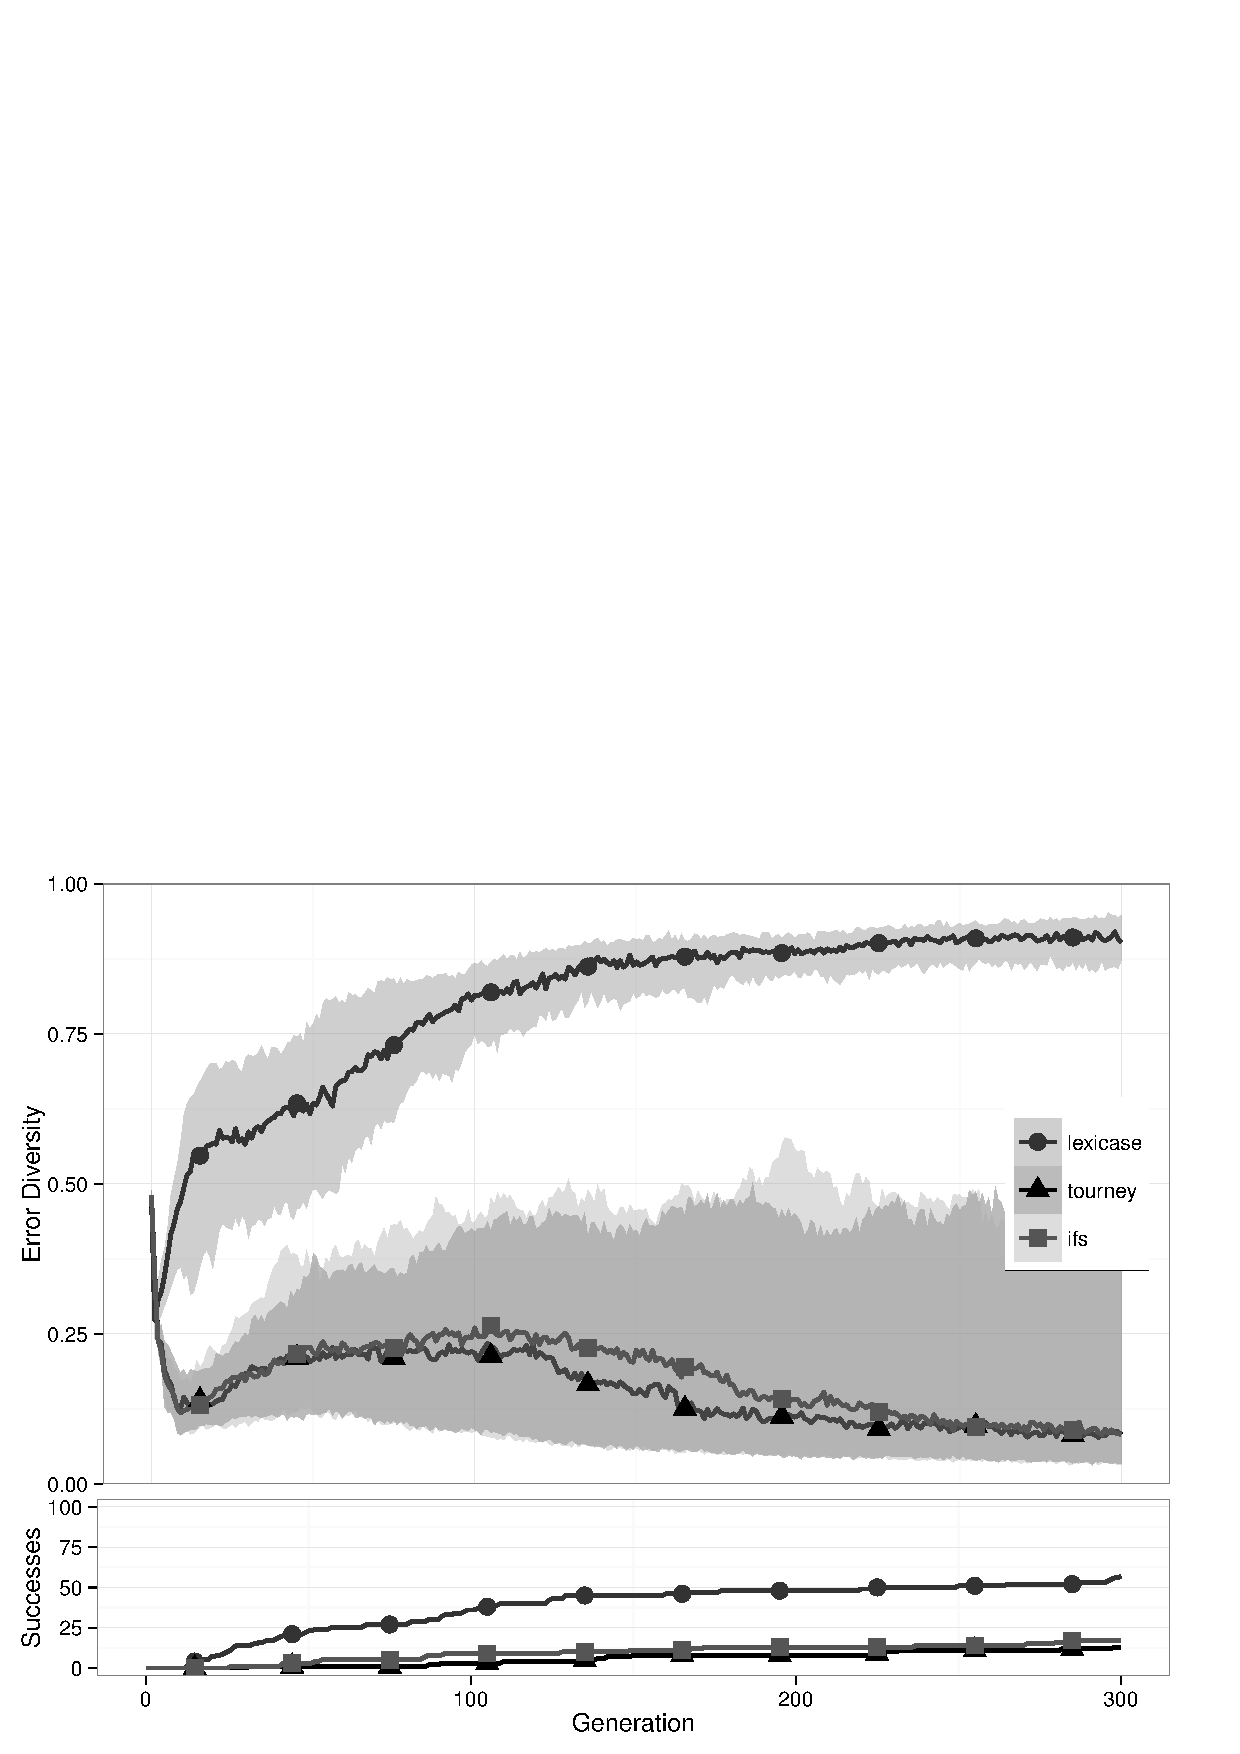
\includegraphics[width=11.5cm]{replace-space-with-newline-diversity.pdf}
\caption{Replace Space With Newline -- error diversity.}
\label{rswnDiv}
\end{figure}

\begin{figure}%[t] %[t] sets the image at the top of the page; t = top, b = bottom, h = here%
%\sidecaption[t]
\centering
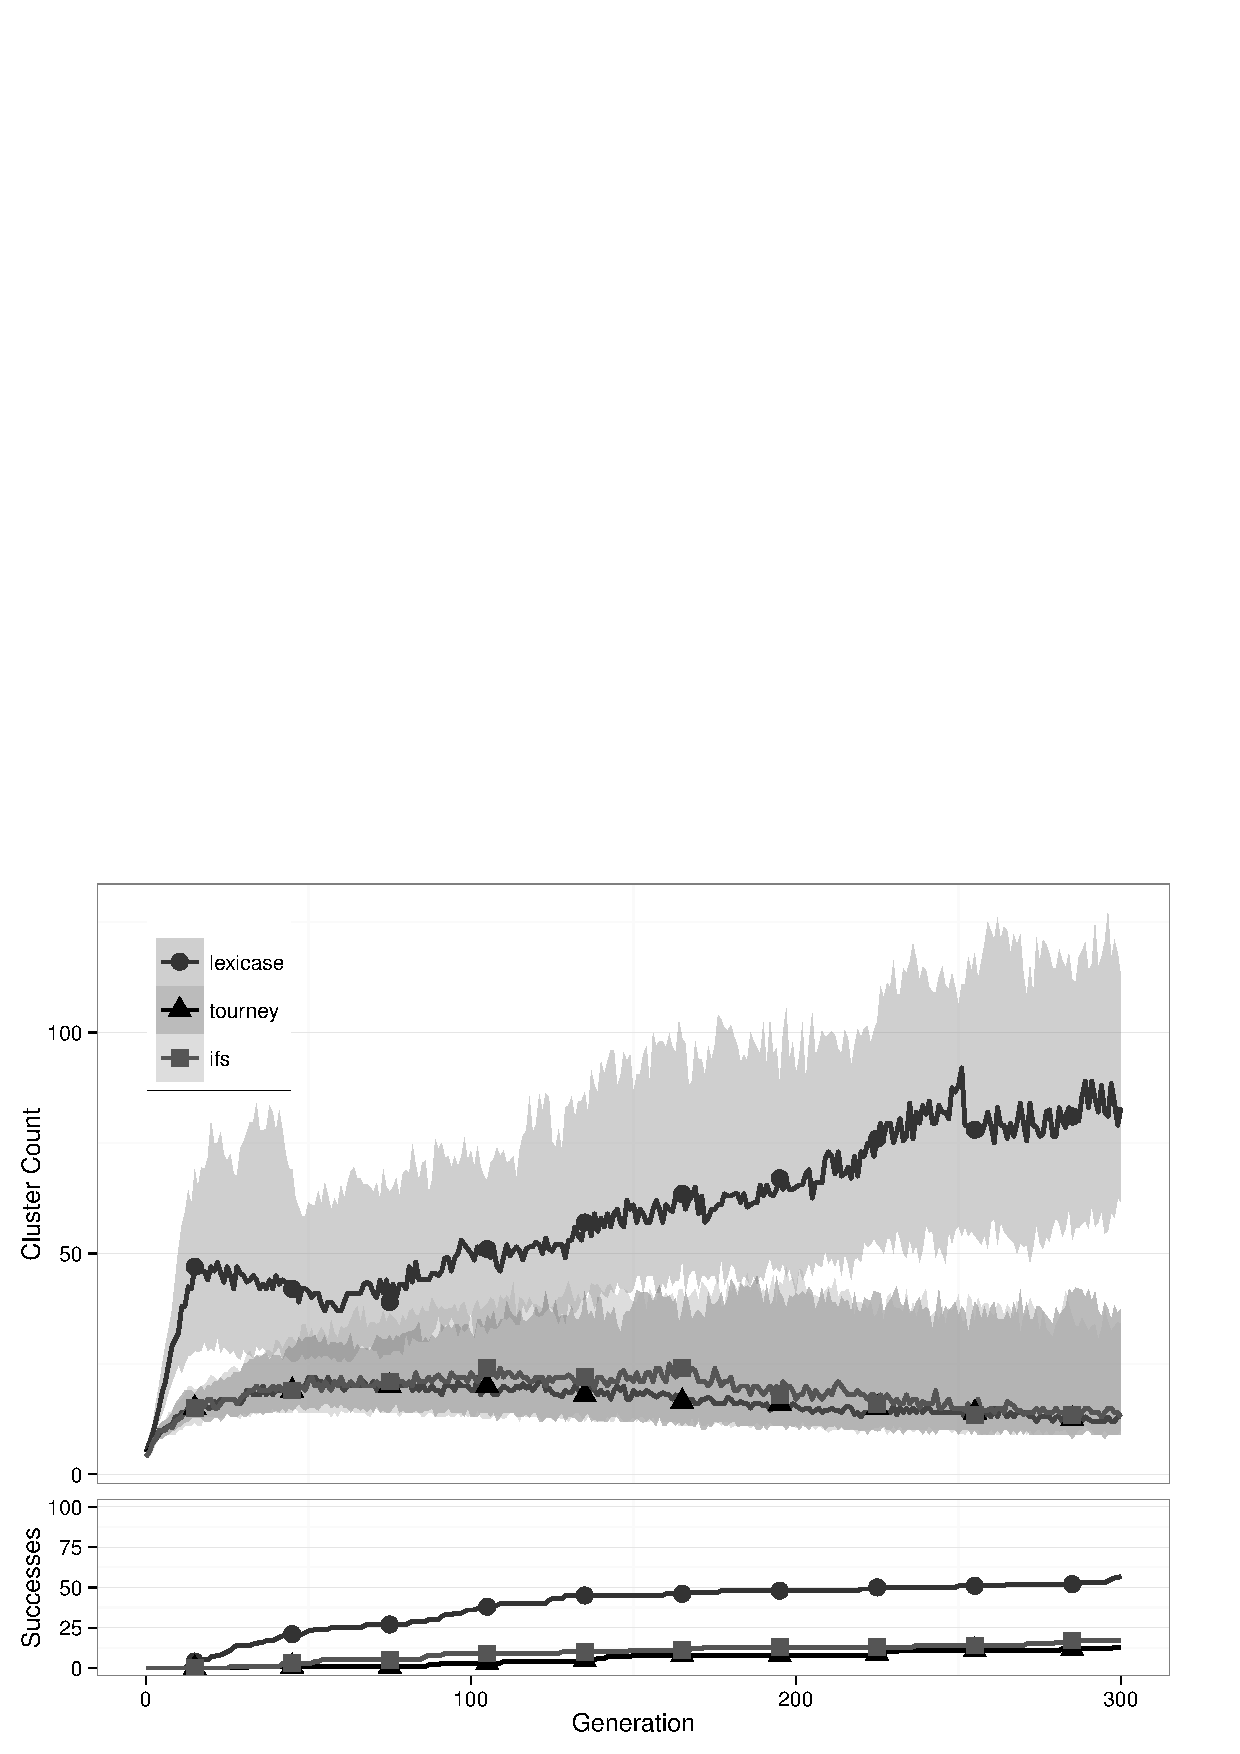
\includegraphics[width=11.5cm]{replace-space-with-newline-cluster.pdf}
\caption{Replace Space With Newline -- clusters.}
\label{rswnClu}
\end{figure}

\begin{figure}%[t] %[t] sets the image at the top of the page; t = top, b = bottom, h = here%
%\sidecaption[t]
\centering
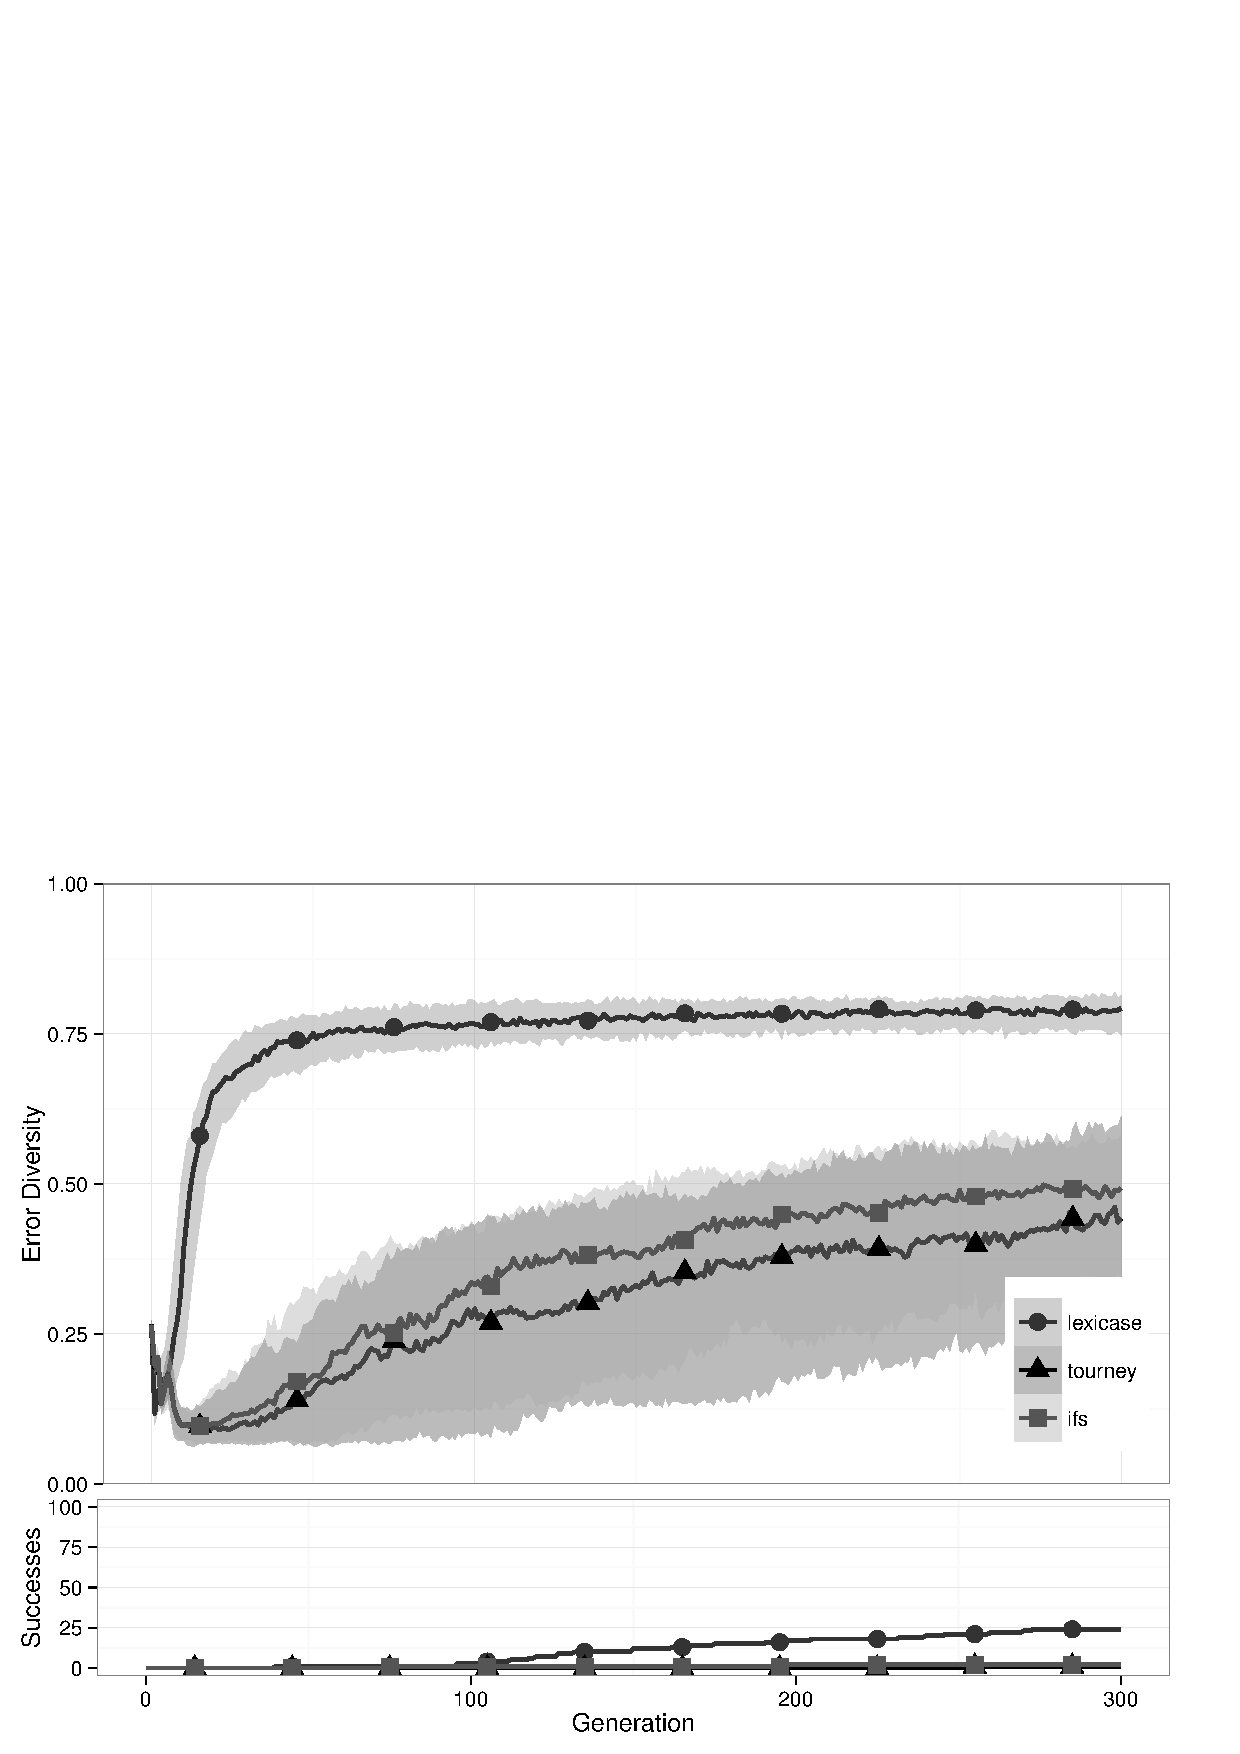
\includegraphics[width=11.5cm]{syllables-diversity.pdf}
\caption{syllables -- error diversity.}
\label{syllablesDiv}
\end{figure}

\begin{figure}%[t] %[t] sets the image at the top of the page; t = top, b = bottom, h = here%
%\sidecaption[t]
\centering
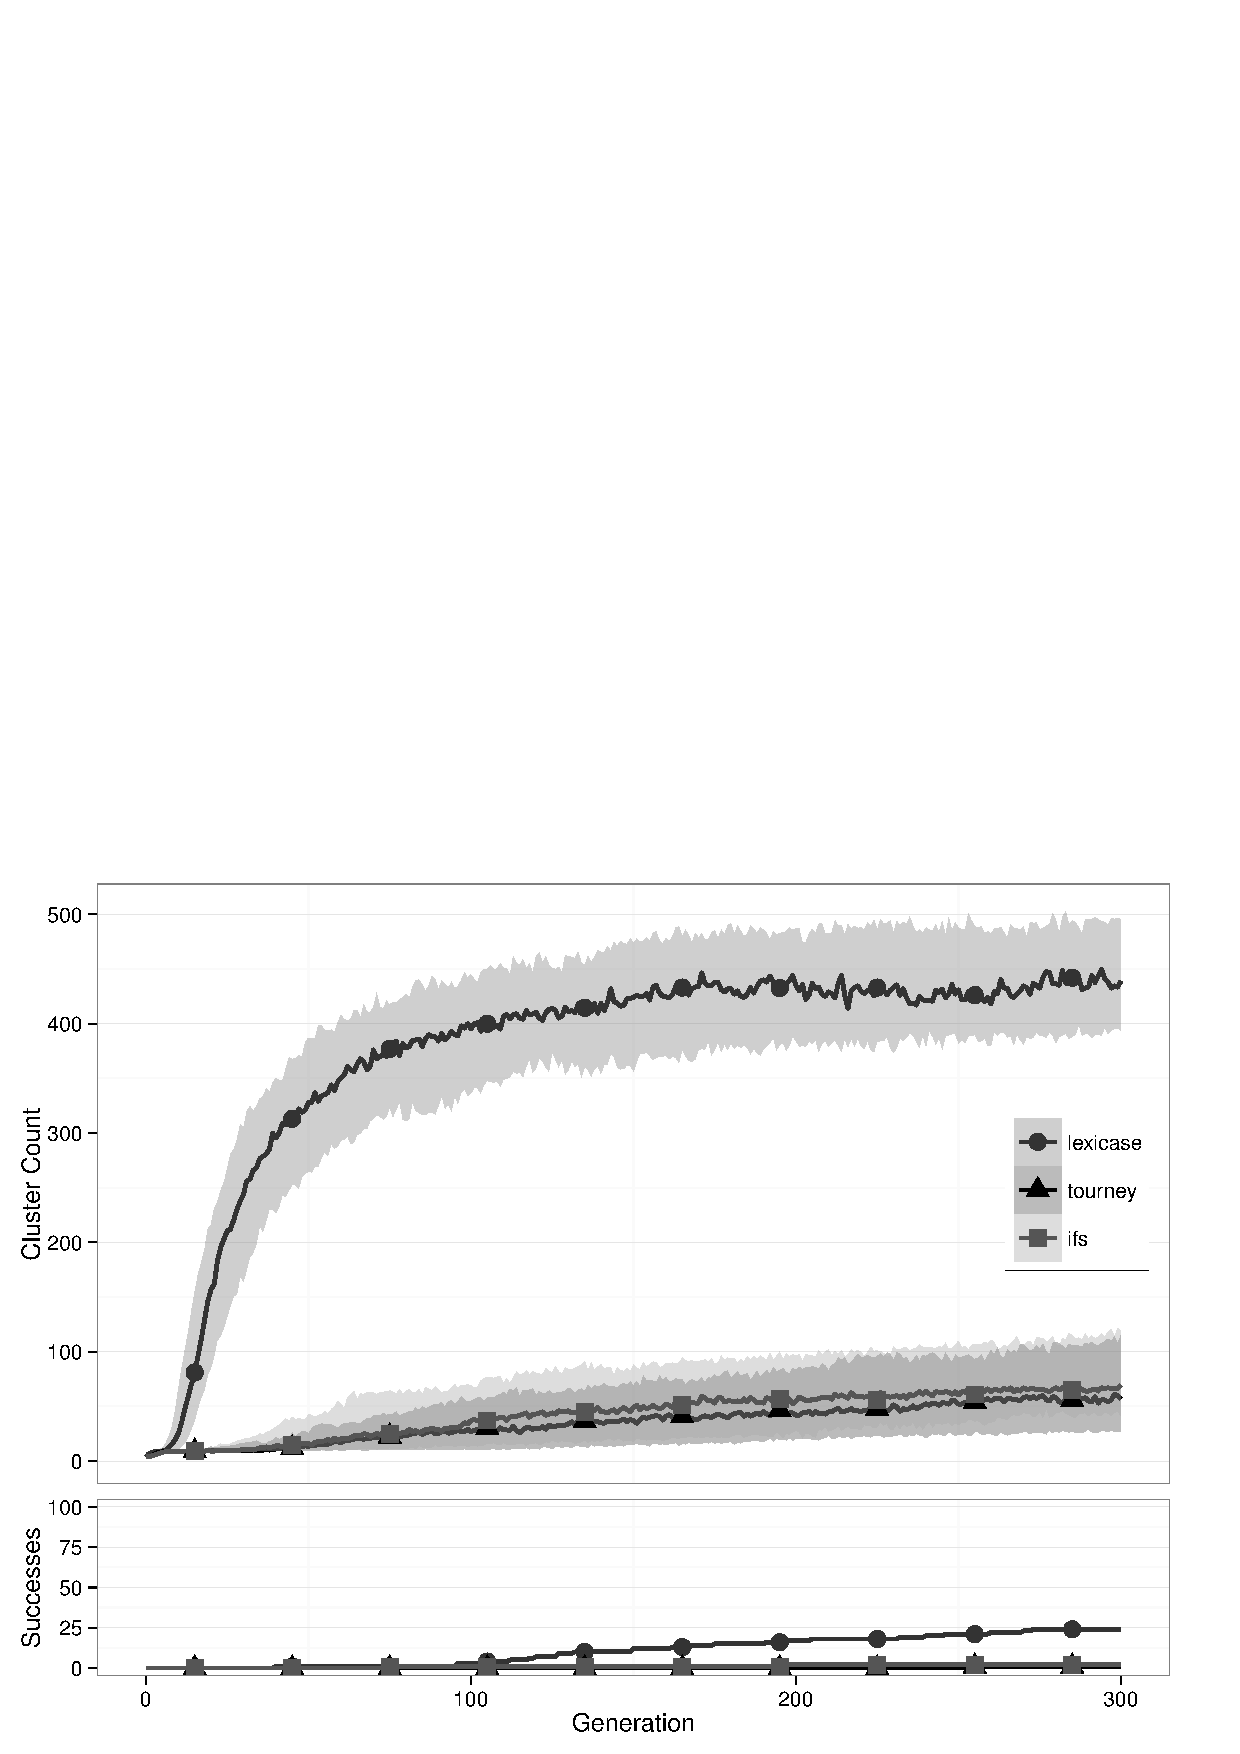
\includegraphics[width=11.5cm]{syllables-cluster.pdf}
\caption{syllables -- clusters.}
\label{syllablesClu}
\end{figure}

\begin{figure}%[t] %[t] sets the image at the top of the page; t = top, b = bottom, h = here%
%\sidecaption[t]
\centering
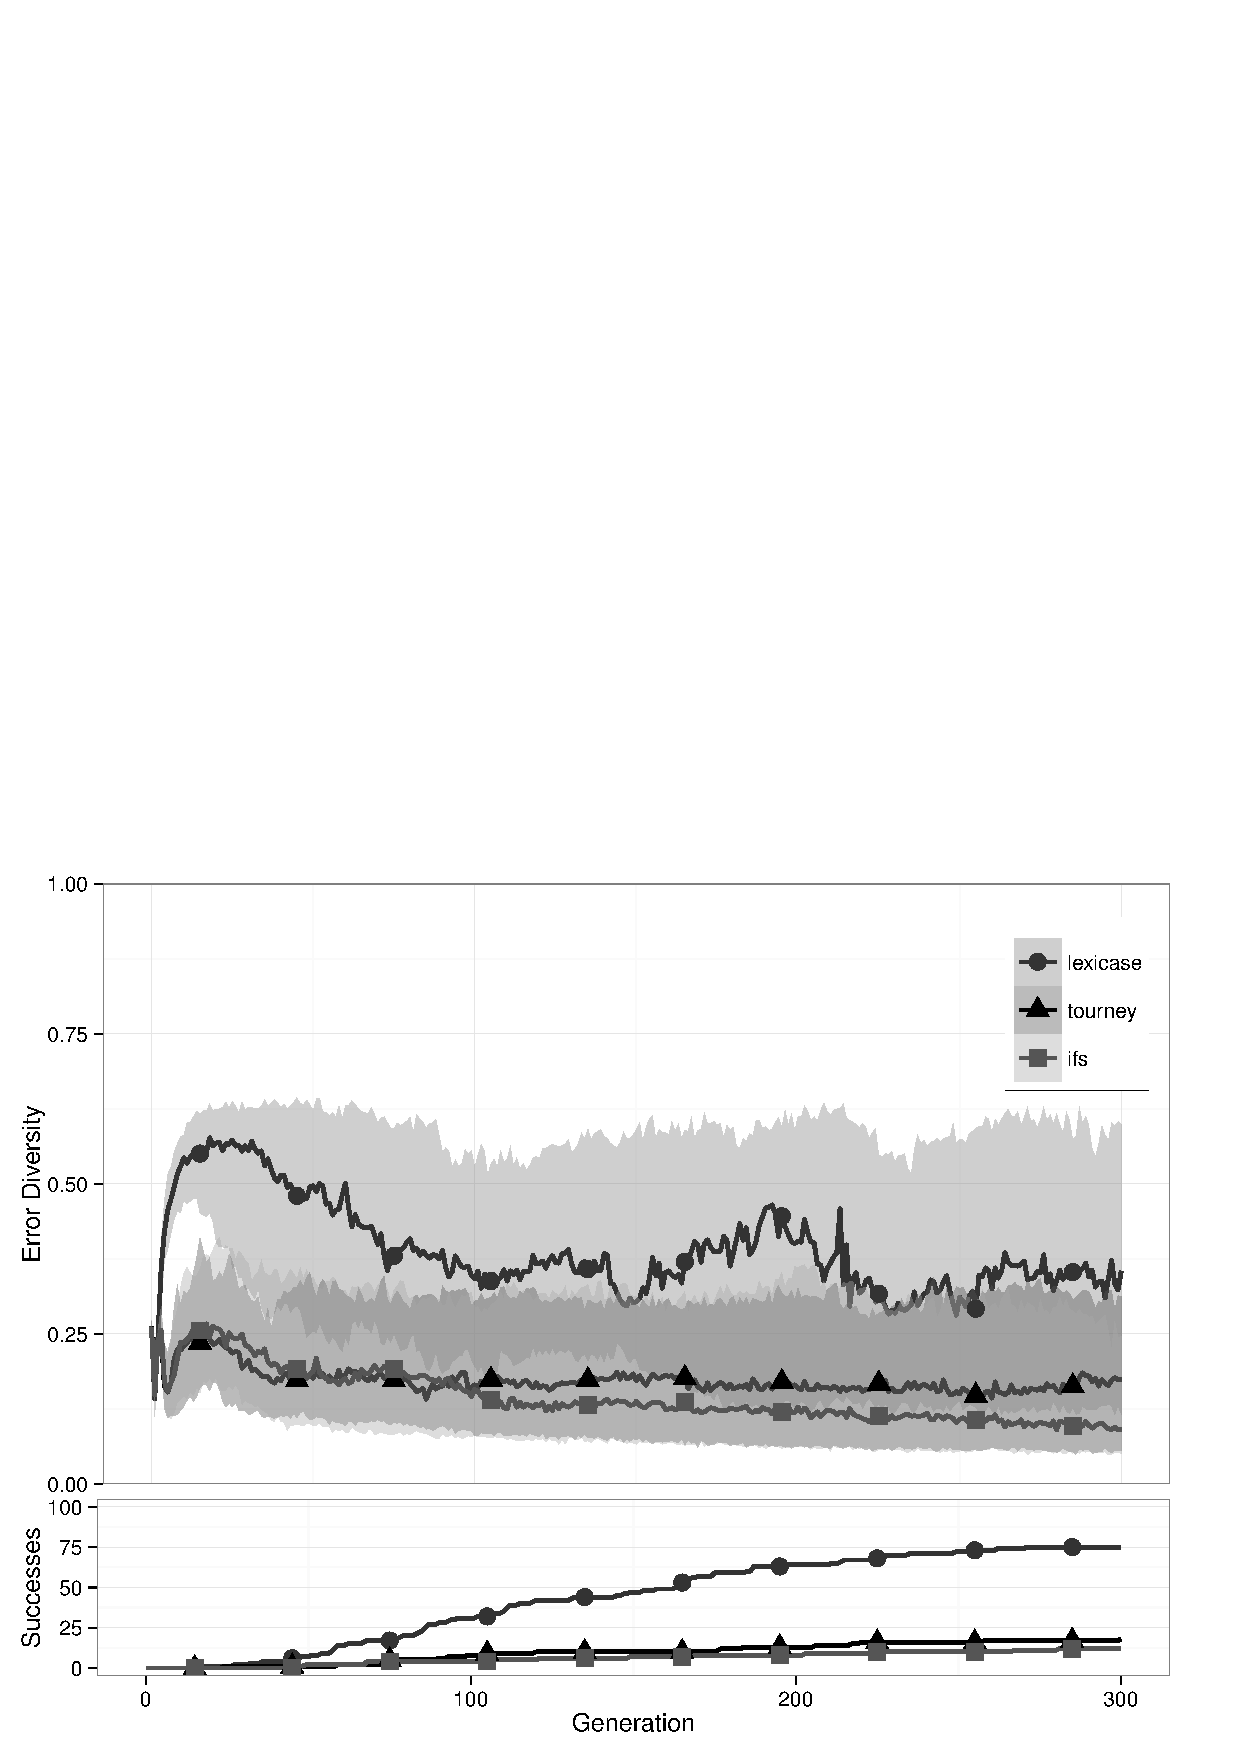
\includegraphics[width=11.5cm]{string-lengths-backwards-diversity.pdf}
\caption{string-lengths-backwards -- error diversity.}
\label{string-lengths-backwardsDiv}
\end{figure}

\begin{figure}%[t] %[t] sets the image at the top of the page; t = top, b = bottom, h = here%
%\sidecaption[t]
\centering
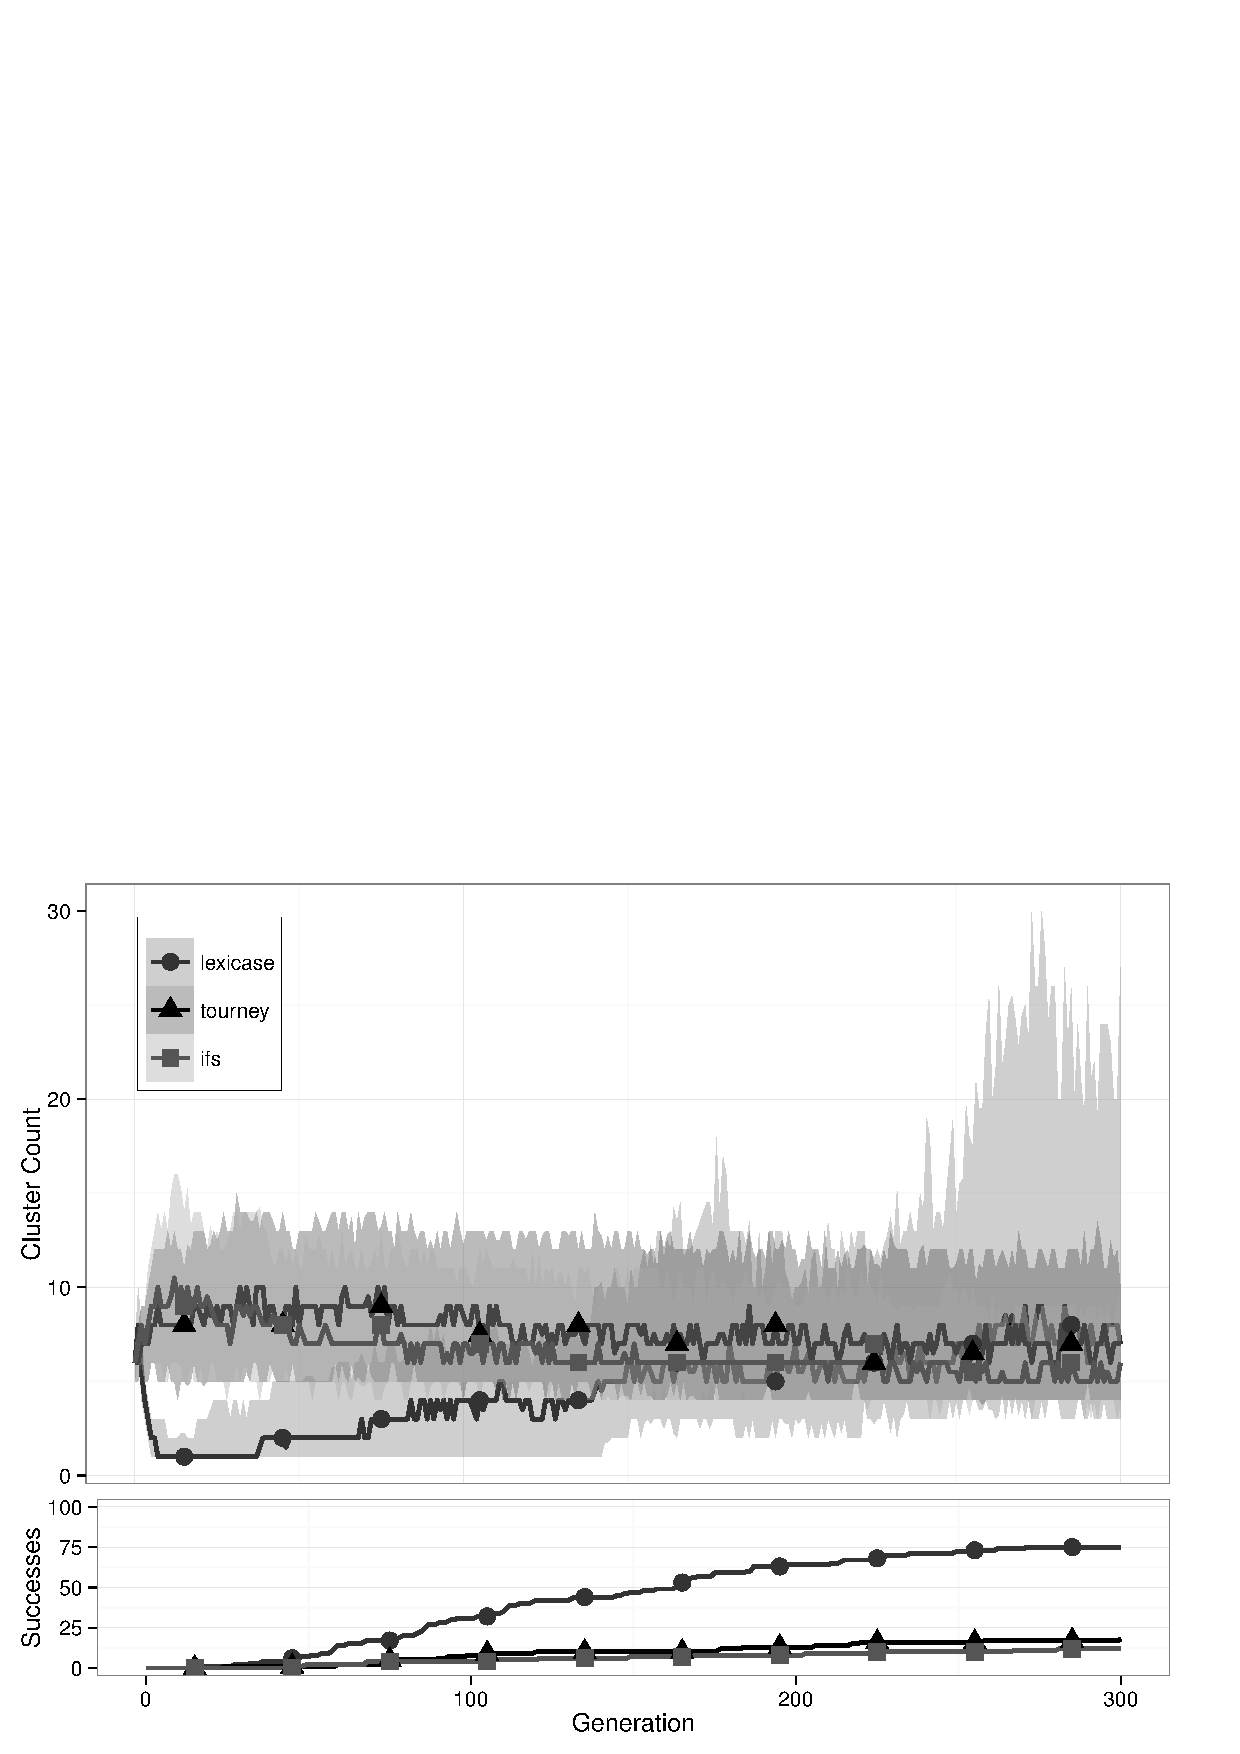
\includegraphics[width=11.5cm]{string-lengths-backwards-cluster.pdf}
\caption{string-lengths-backwards -- clusters.}
\label{string-lengths-backwardsClu}
\end{figure}

\begin{figure}%[t] %[t] sets the image at the top of the page; t = top, b = bottom, h = here%
%\sidecaption[t]
\centering
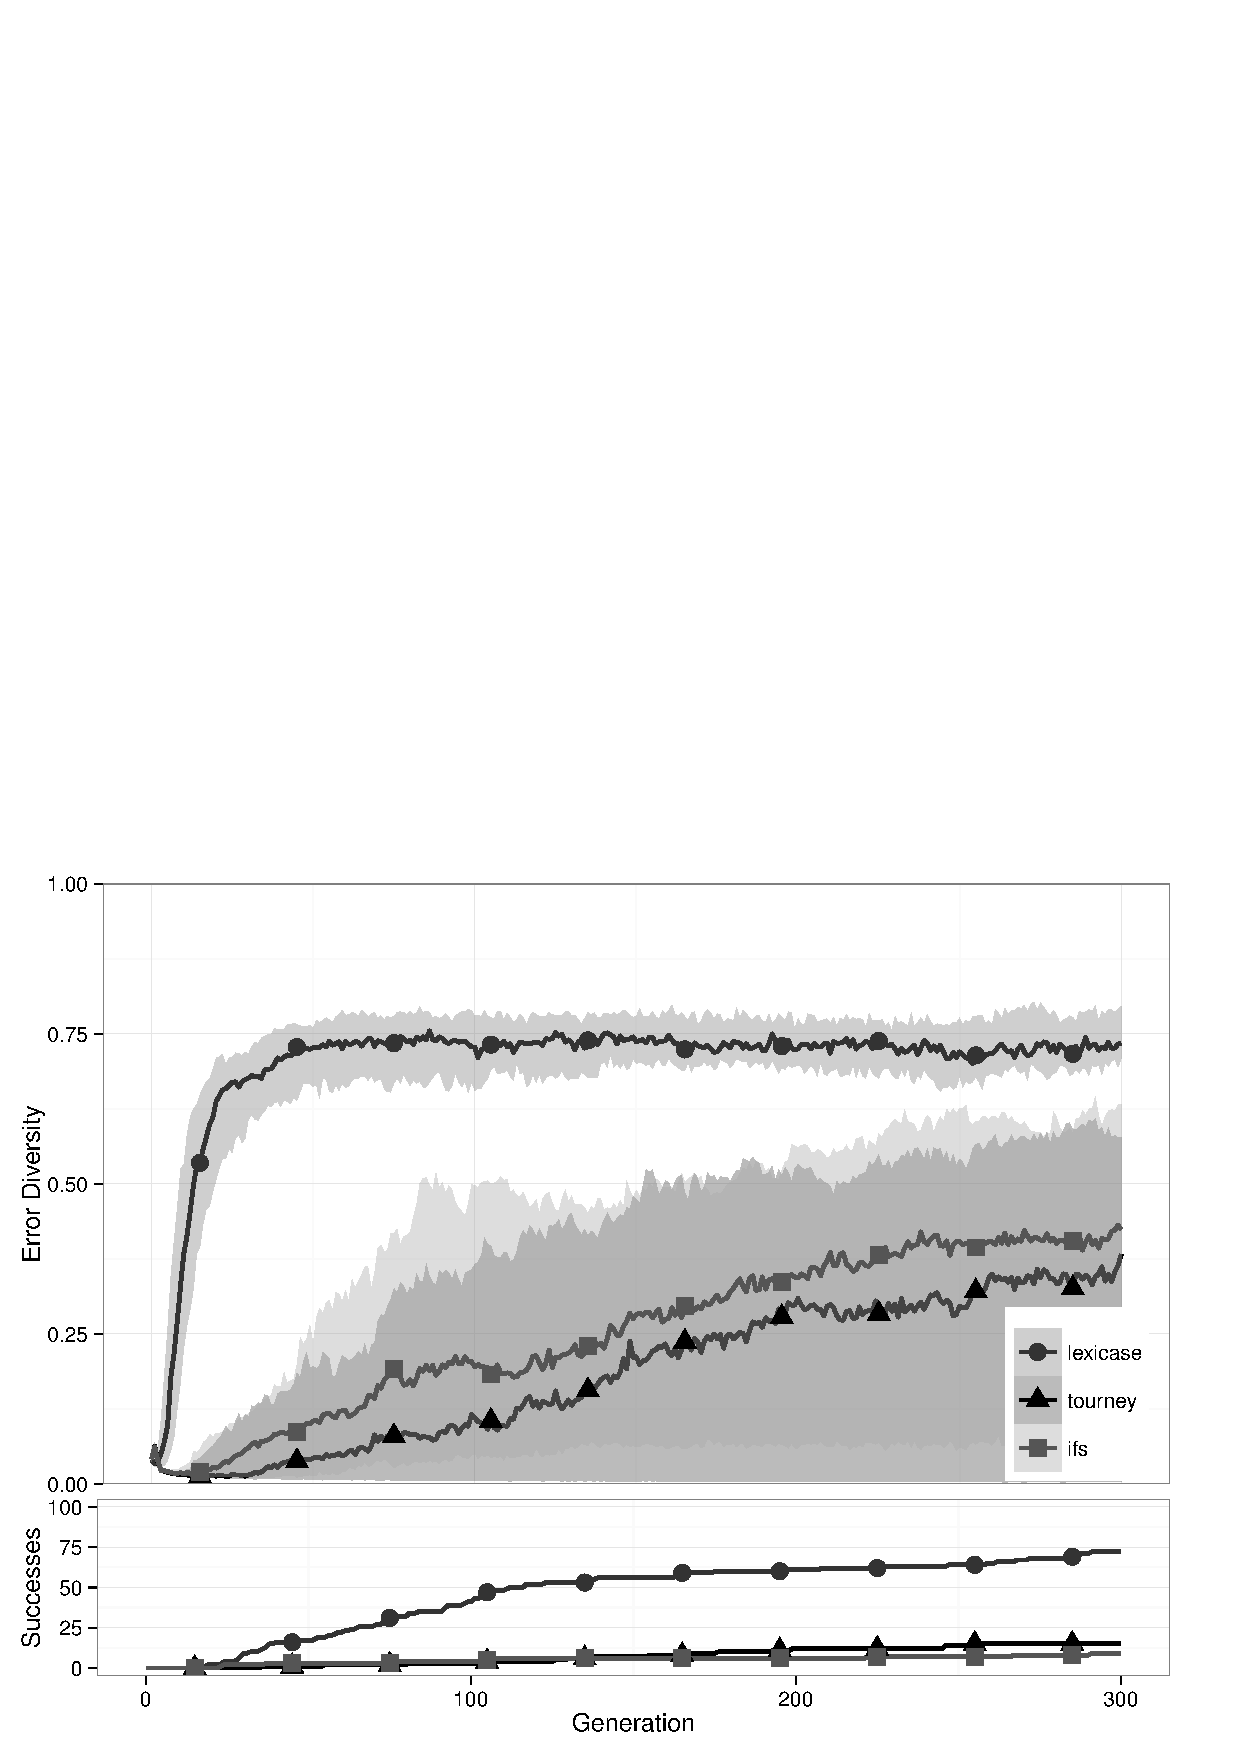
\includegraphics[width=11.5cm]{negative-to-zero-diversity.pdf}
\caption{negative-to-zero -- error diversity.}
\label{negative-to-zeroDiv}
\end{figure}

\begin{figure}%[t] %[t] sets the image at the top of the page; t = top, b = bottom, h = here%
%\sidecaption[t]
\centering
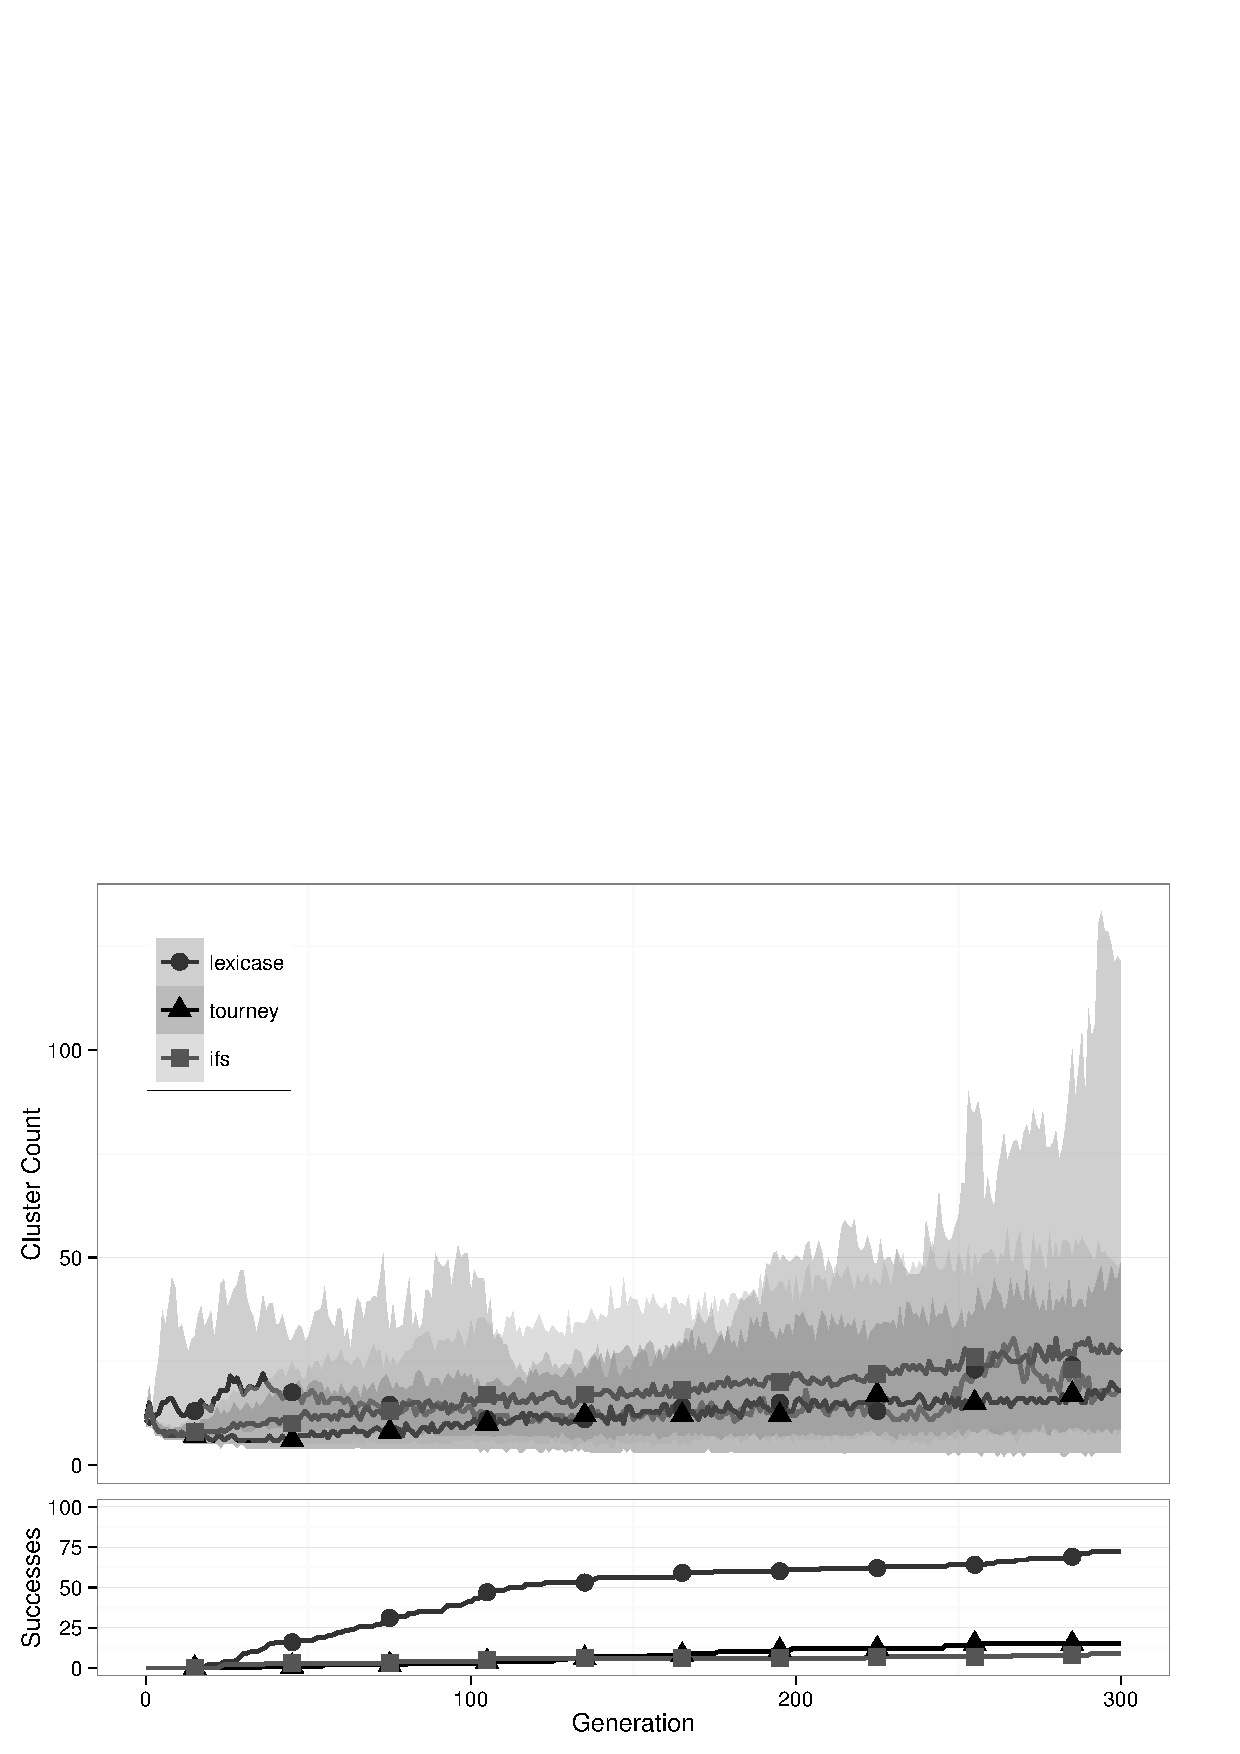
\includegraphics[width=11.5cm]{negative-to-zero-cluster.pdf}
\caption{negative-to-zero -- clusters.}
\label{negative-to-zeroClu}
\end{figure}

\begin{figure}%[t] %[t] sets the image at the top of the page; t = top, b = bottom, h = here%
%\sidecaption[t]
\centering
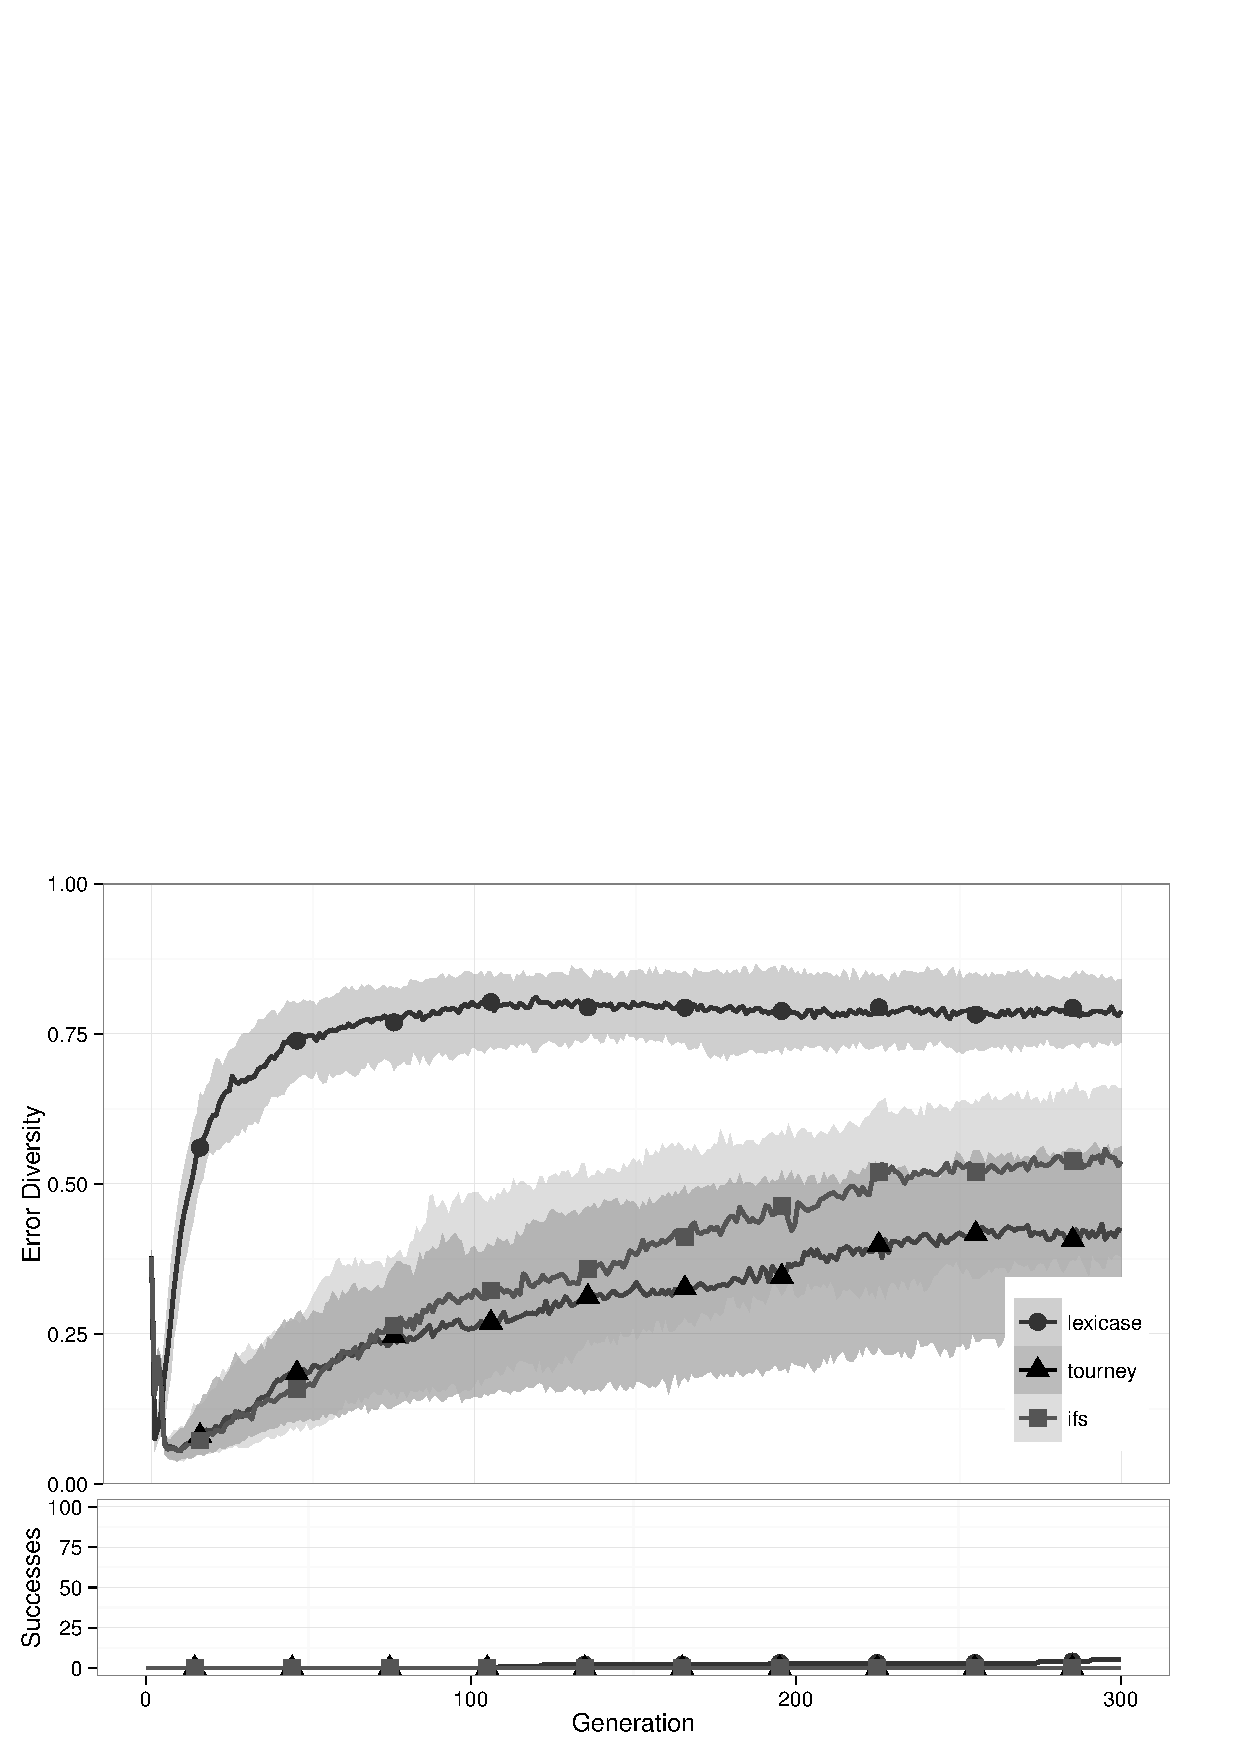
\includegraphics[width=11.5cm]{double-letters-diversity.pdf}
\caption{double-letters -- error diversity.}
\label{double-lettersDiv}
\end{figure}

\begin{figure}%[t] %[t] sets the image at the top of the page; t = top, b = bottom, h = here%
%\sidecaption[t]
\centering
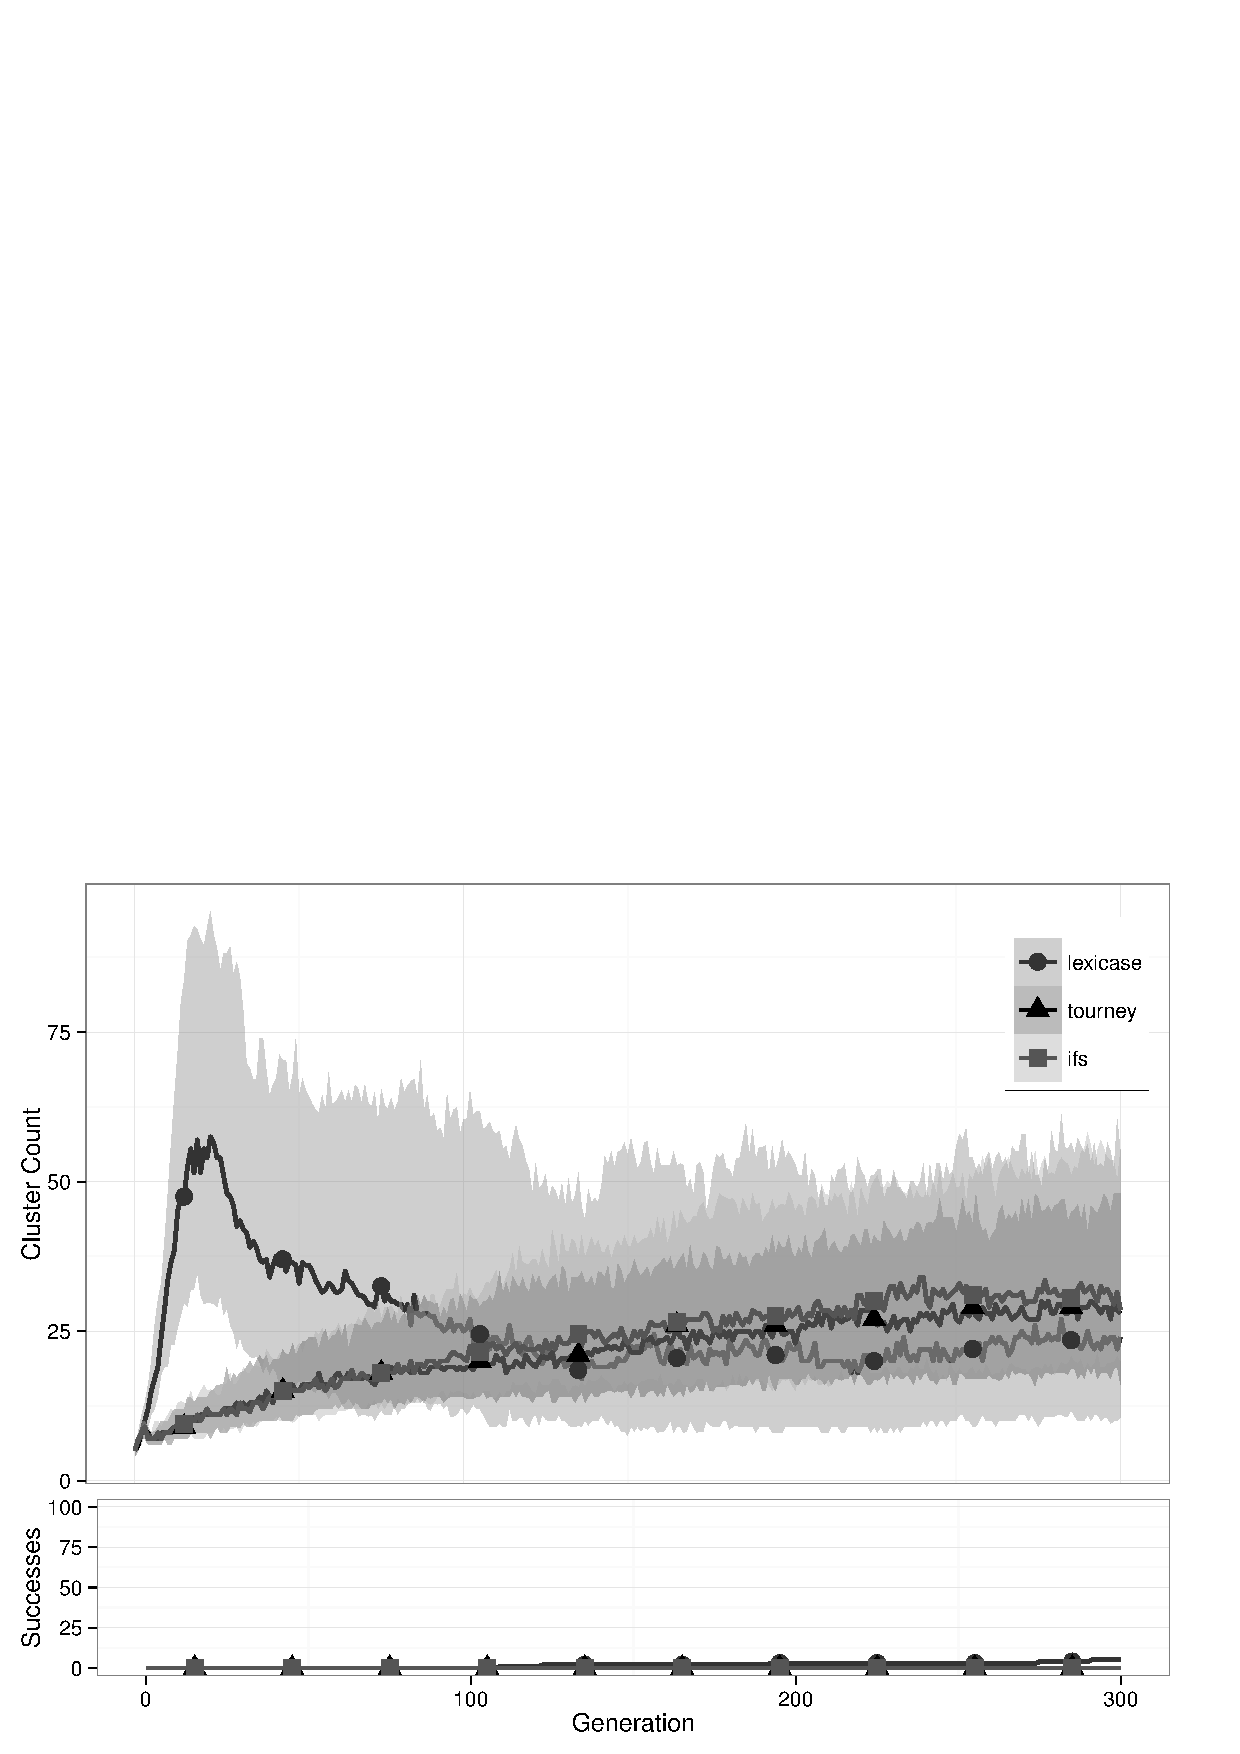
\includegraphics[width=11.5cm]{double-letters-cluster.pdf}
\caption{double-letters -- clusters.}
\label{double-lettersClu}
\end{figure}

\begin{figure}%[t] %[t] sets the image at the top of the page; t = top, b = bottom, h = here%
%\sidecaption[t]
\centering
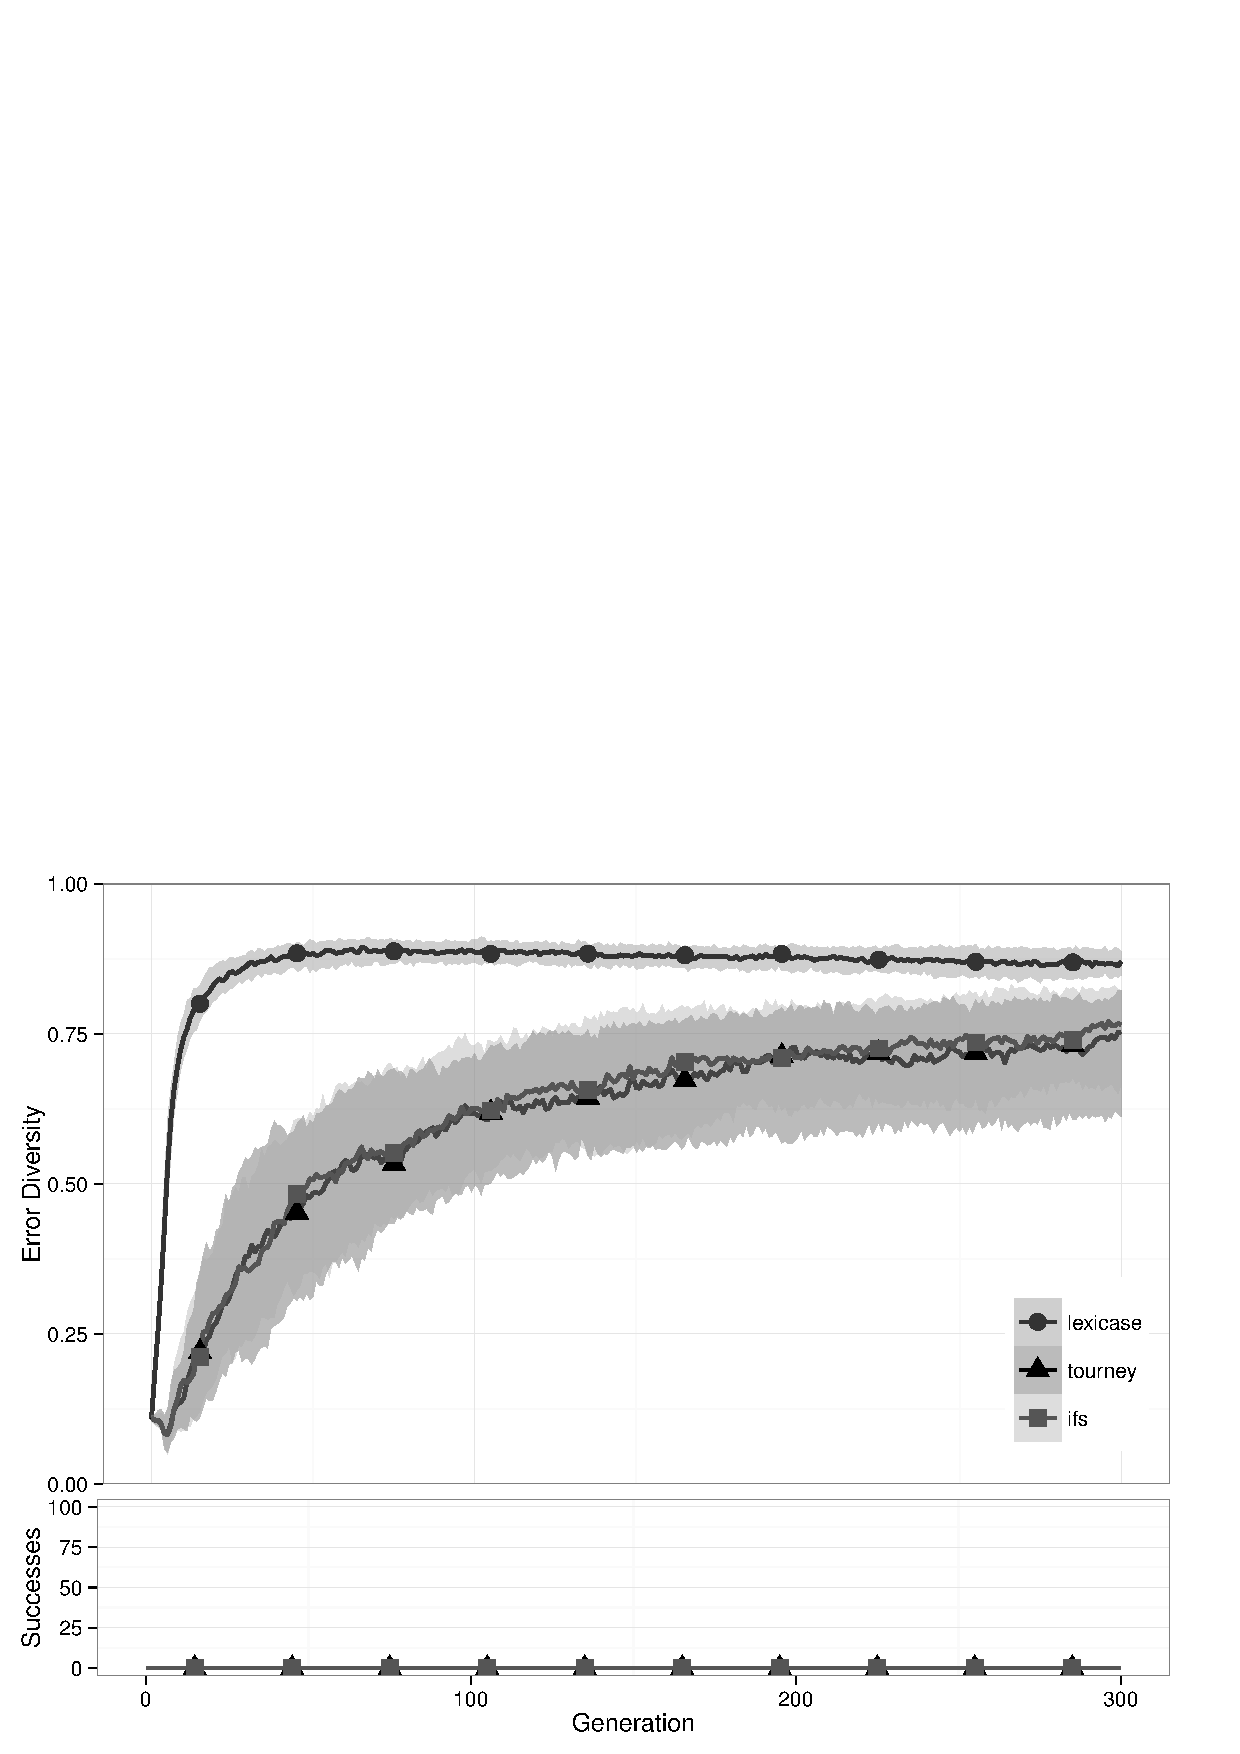
\includegraphics[width=11.5cm]{scrabble-score-diversity.pdf}
\caption{scrabble-score -- error diversity.}
\label{scrabble-scoreDiv}
\end{figure}

\begin{figure}%[t] %[t] sets the image at the top of the page; t = top, b = bottom, h = here%
%\sidecaption[t]
\centering
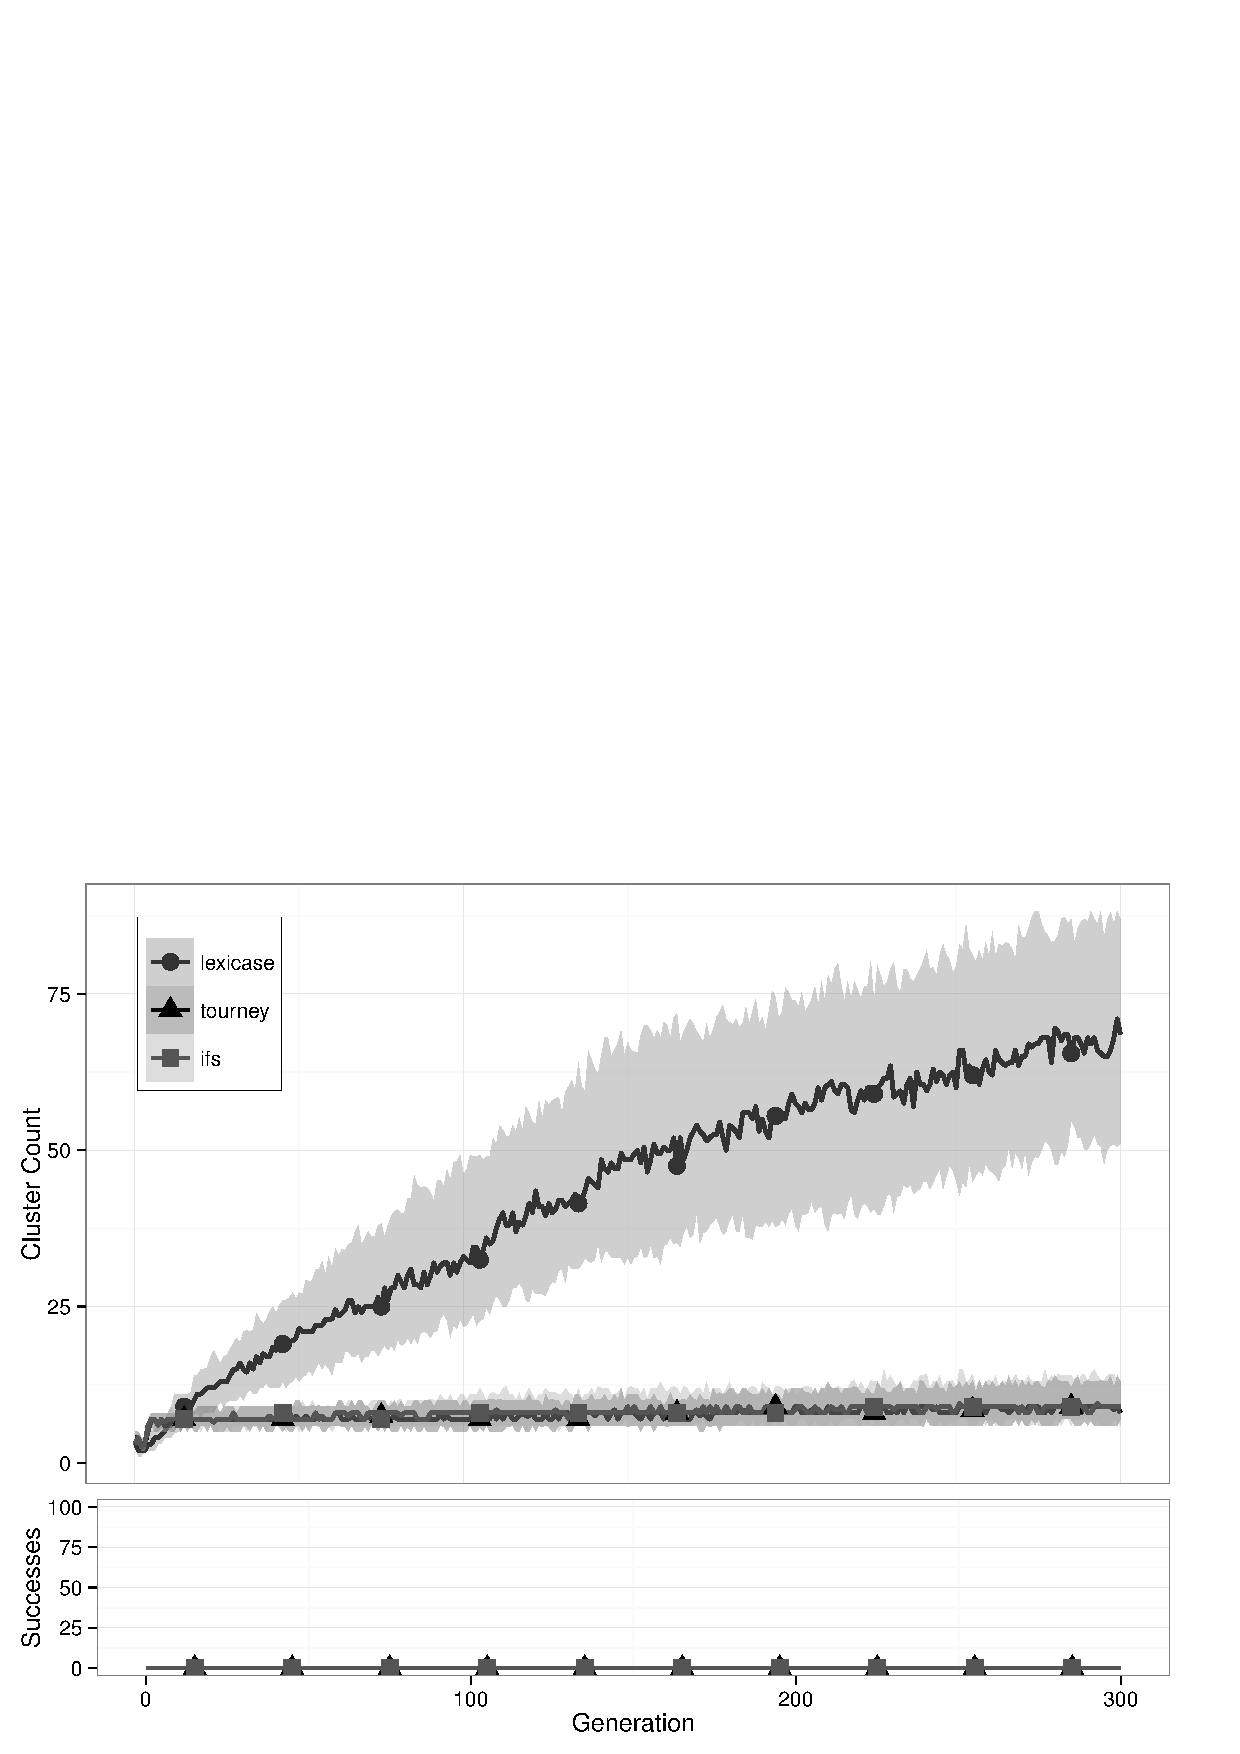
\includegraphics[width=11.5cm]{scrabble-score-cluster.pdf}
\caption{scrabble-score -- clusters.}
\label{scrabble-scoreClu}
\end{figure}

\begin{figure}%[t] %[t] sets the image at the top of the page; t = top, b = bottom, h = here%
%\sidecaption[t]
\centering
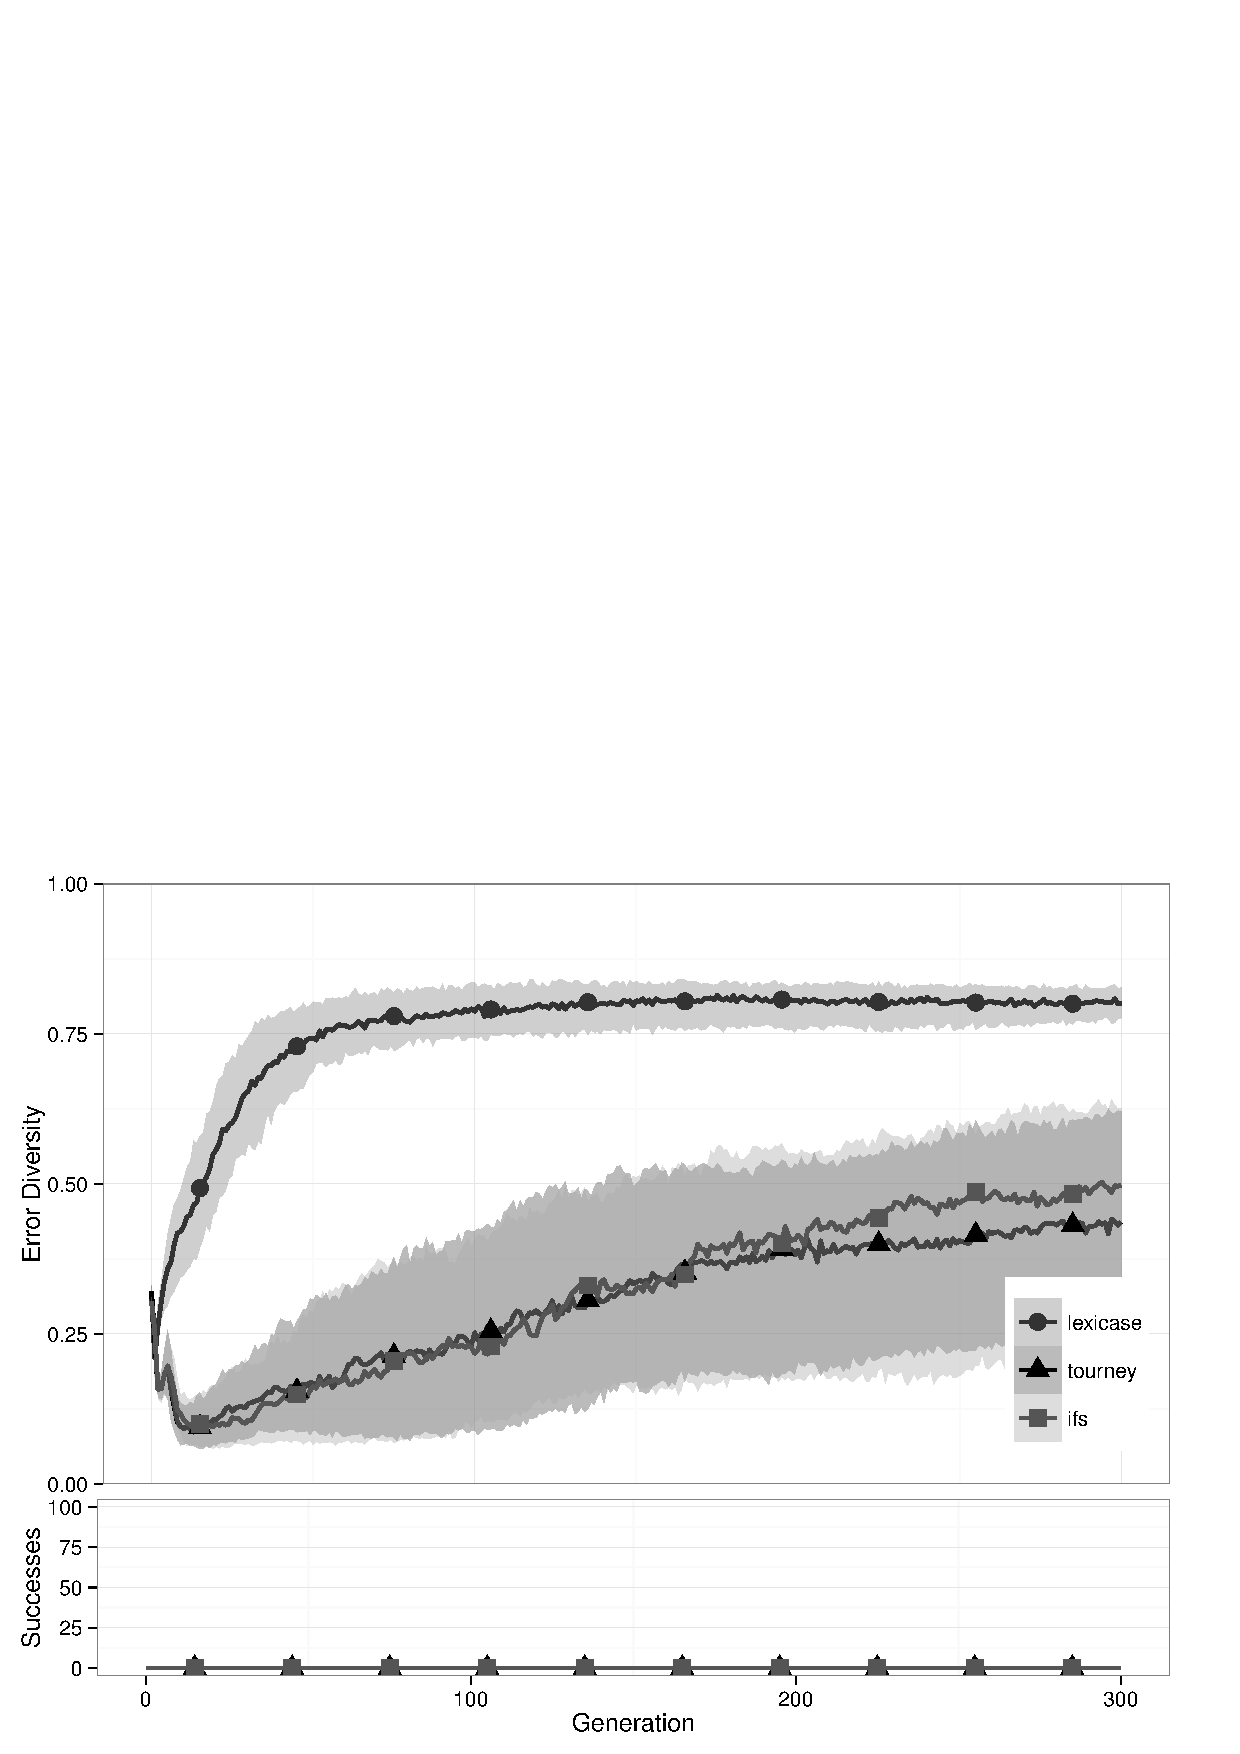
\includegraphics[width=11.5cm]{checksum-diversity.pdf}
\caption{checksum -- error diversity.}
\label{checksumDiv}
\end{figure}

\begin{figure}%[t] %[t] sets the image at the top of the page; t = top, b = bottom, h = here%
%\sidecaption[t]
\centering
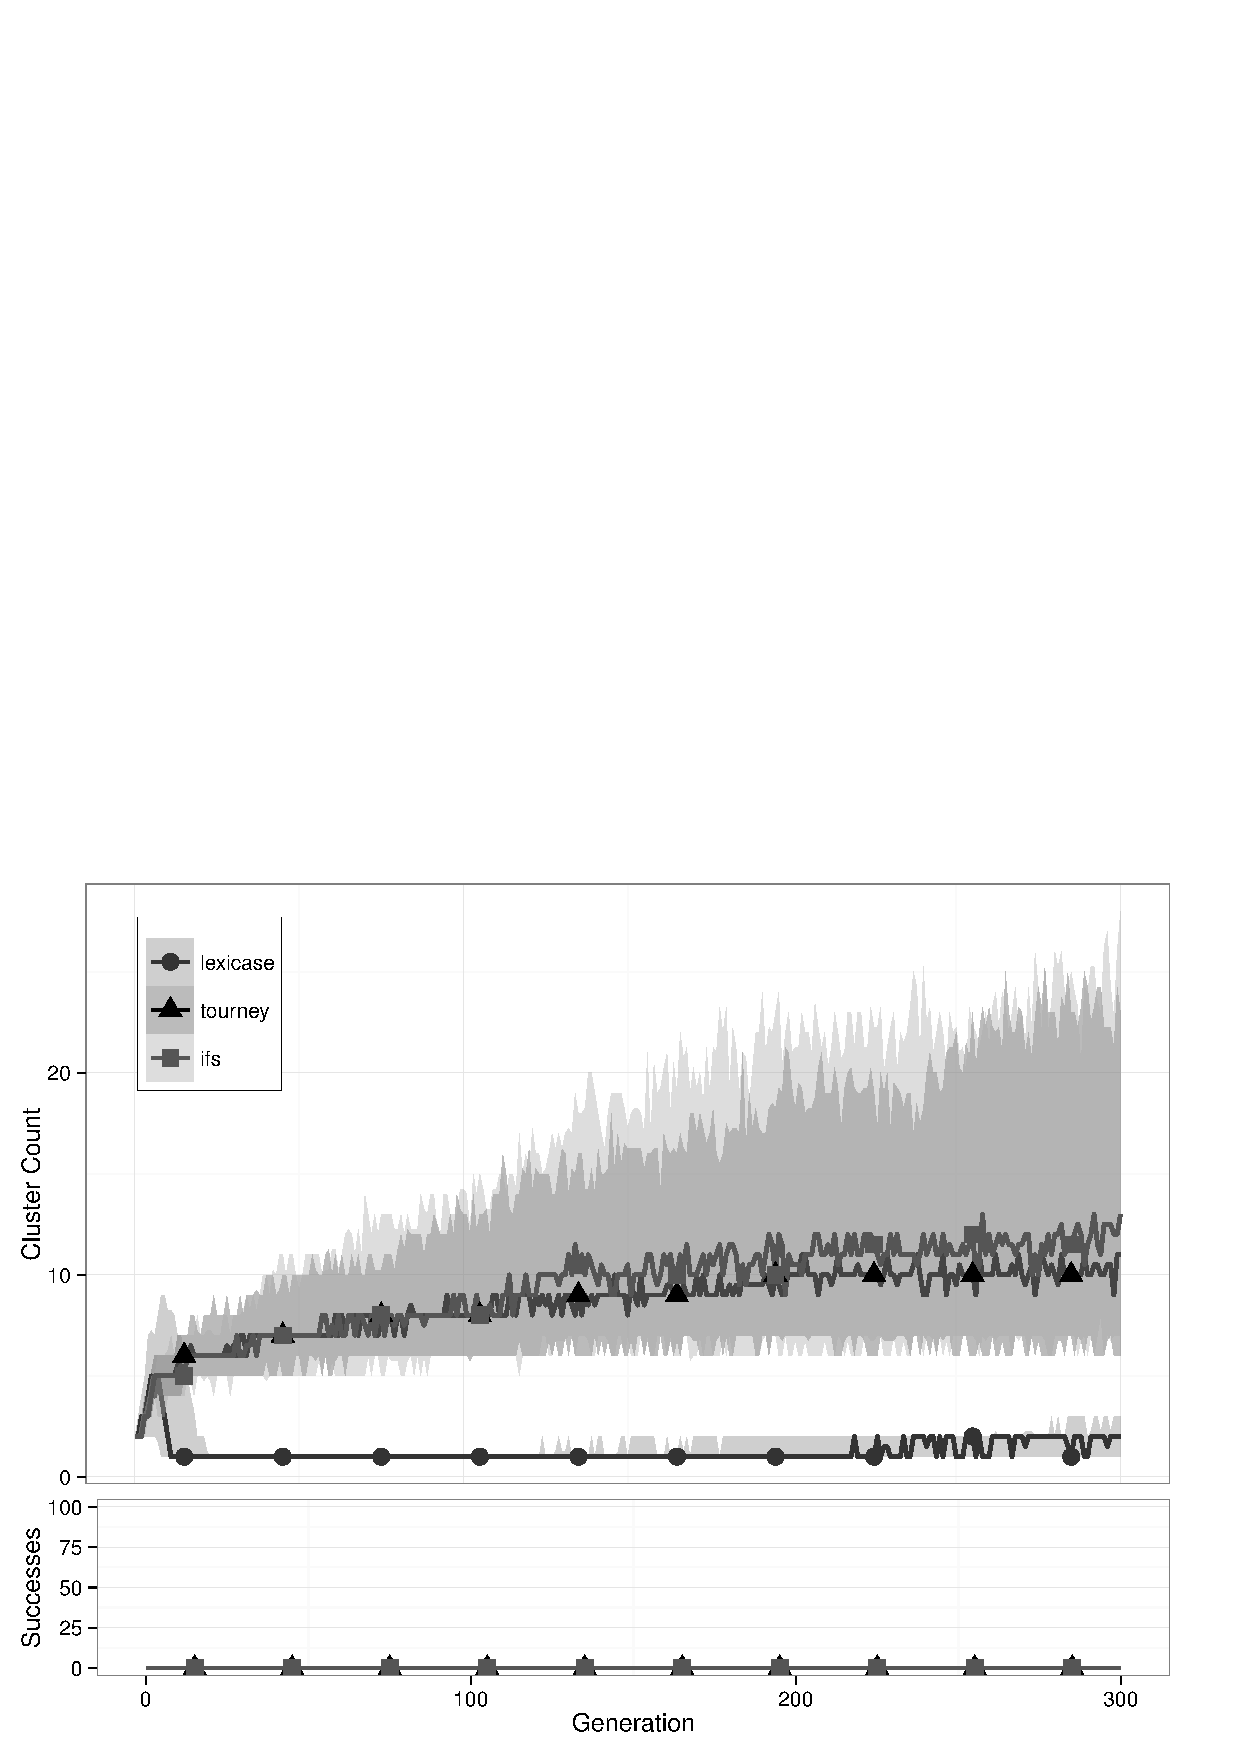
\includegraphics[width=11.5cm]{checksum-cluster.pdf}
\caption{checksum -- clusters.}
\label{checksumClu}
\end{figure}

\begin{figure}%[t] %[t] sets the image at the top of the page; t = top, b = bottom, h = here%
%\sidecaption[t]
\centering
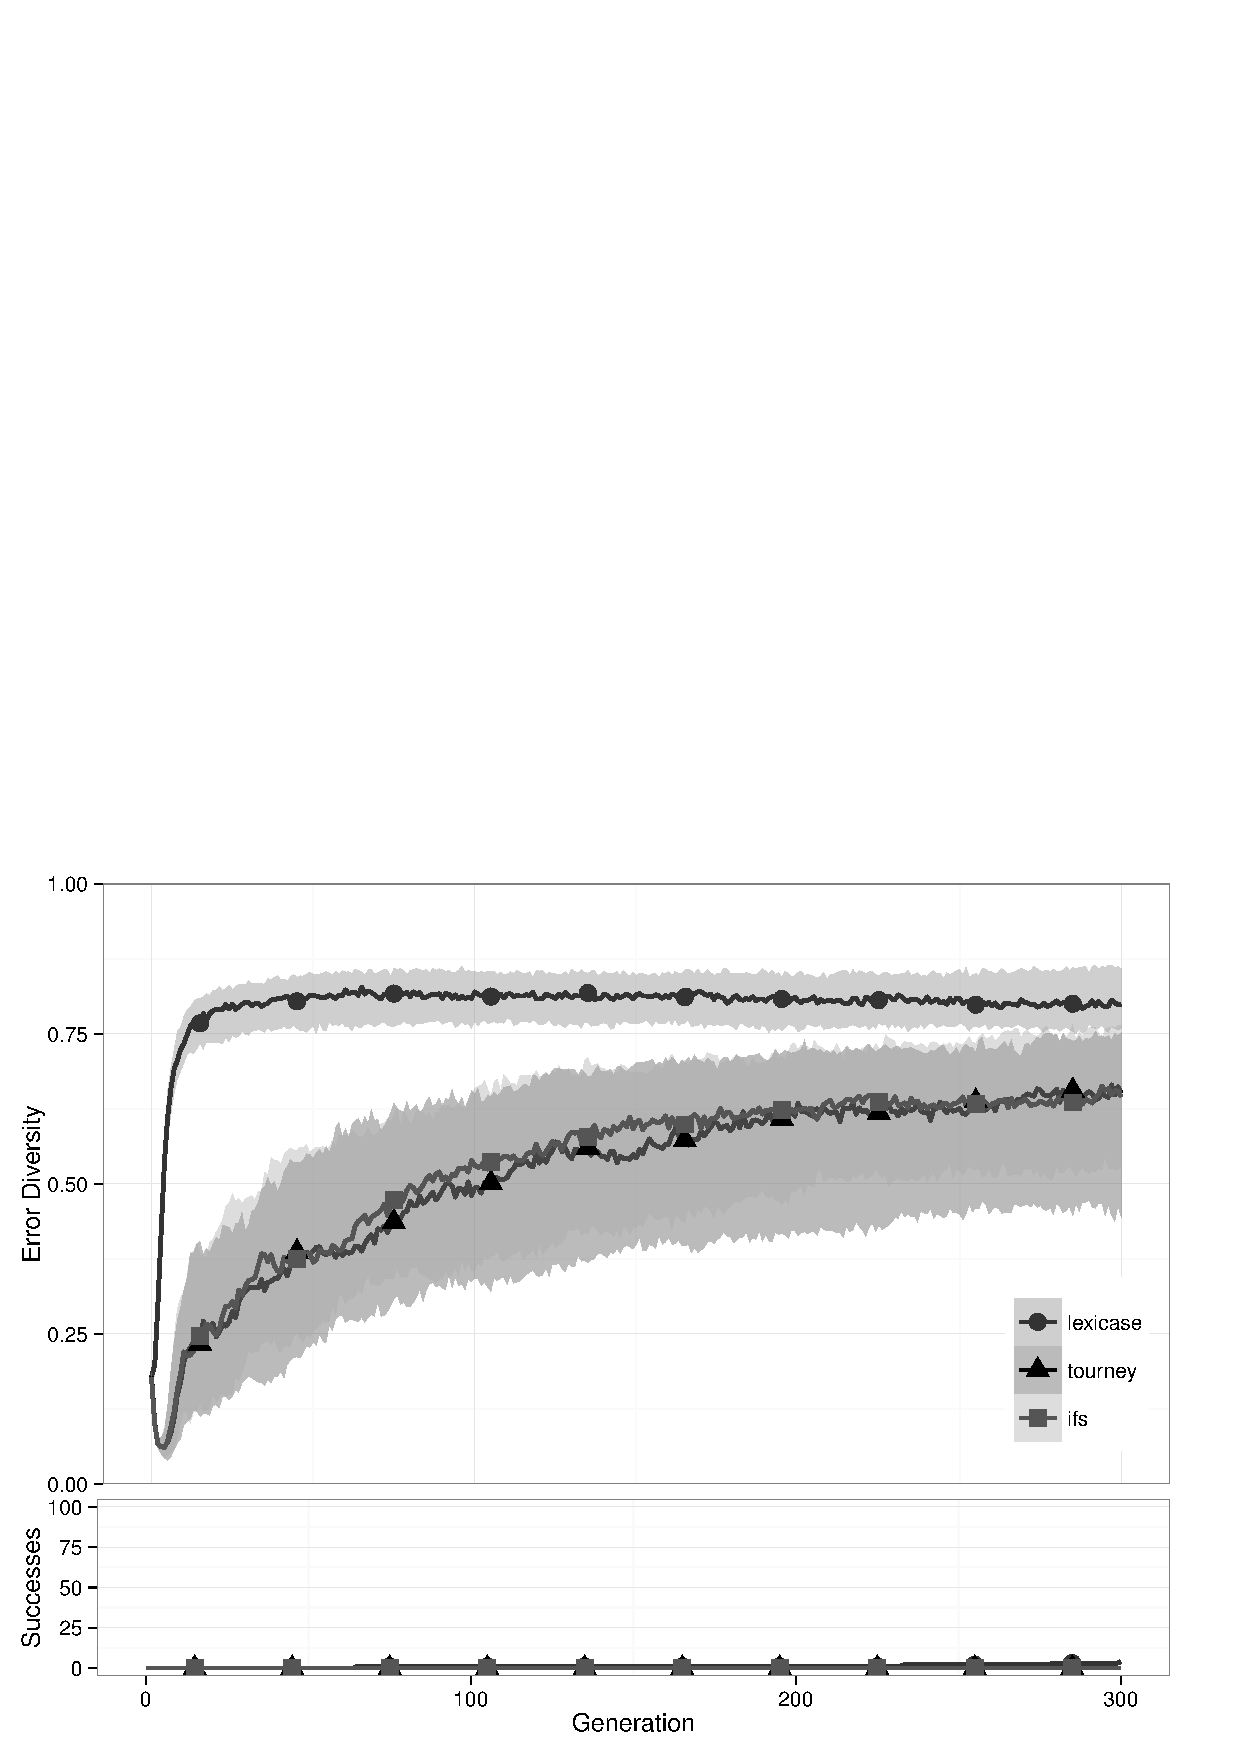
\includegraphics[width=11.5cm]{count-odds-diversity.pdf}
\caption{count-odds -- error diversity.}
\label{count-oddsDiv}
\end{figure}

\begin{figure}%[t] %[t] sets the image at the top of the page; t = top, b = bottom, h = here%
%\sidecaption[t]
\centering
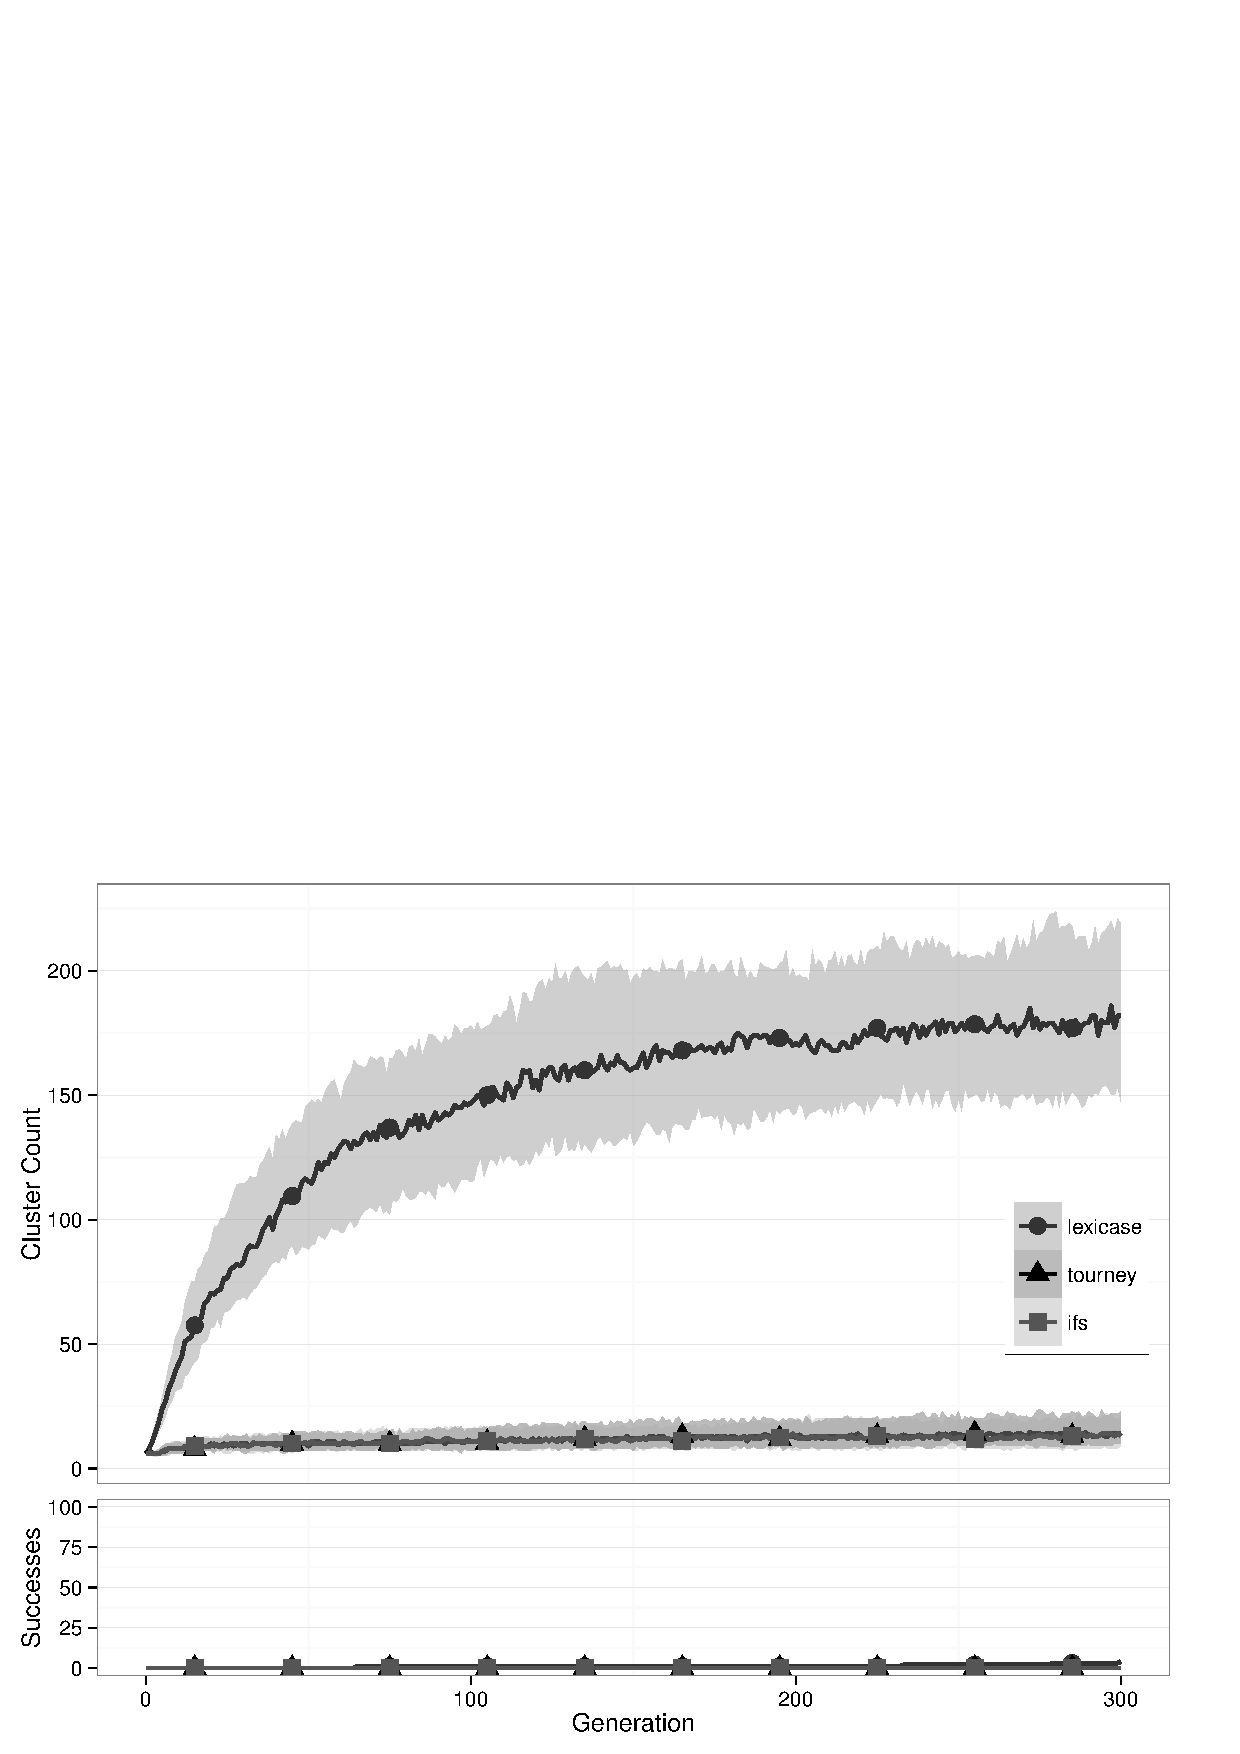
\includegraphics[width=11.5cm]{count-odds-cluster.pdf}
\caption{count-odds -- clusters.}
\label{count-oddsClu}
\end{figure}


\section{Discussion and importance of findings}

(include correlation with better success rates with lexicase)

\section{Conclusions}


\begin{acknowledgement}
Added later.
\end{acknowledgement}

\bibliographystyle{spbasic}
\bibliography{gp-bibliography,spector}
